\documentclass[xcolor=table]{beamer}
\usepackage[utf8]{inputenc}
\usepackage{listings}
\usepackage{adjustbox}
\usepackage{graphicx}
\usepackage{wrapfig}
\usepackage{tikz}  
\usepackage[norsk]{babel}
\usepackage{caption}
\captionsetup{font=scriptsize,labelfont=scriptsize}

\setbeamertemplate{footline}{%
\insertframenumber{}/\inserttotalframenumber}

\usepackage[
    backend=biber,
    style=numeric,
    sorting=none
]{biblatex}
\addbibresource{thesis/refs.bib}

\title[Spoof proof GPS timing] % (optional, only for long titles)
{Spoof proof GPS timing}
\subtitle{A detection and mitigation system for GPS time spoofing}
\author[A. Schultzen] % (optional, for multiple authors)
{A.~Schultzen\inst{1}}
\institute[Universities Here and There] % (optional)
{
  \inst{1}%
  Institutt for informatikk\\
  Universitetet i Oslo
}

\setcounter{tocdepth}{1}
\date{\today}
\usetheme{Marburg}

\begin{document}

\frame{\titlepage}

\section{Introduksjon}
\begin{frame}
  \frametitle{Introduksjon}
  \begin{itemize}
    \setlength\itemsep{2em}
    \item GPS-mottakere er naive, enkle å narre
    \item Enkle tiltak
    \item Laget system for å teste deteksjon og mottiltak
\end{itemize}
\end{frame}

\subsection{GPS timing}
\begin{frame}
  \frametitle{Introduksjon}
\framesubtitle{GPS timing} 
  \begin{figure}
  \vspace{-30pt}
      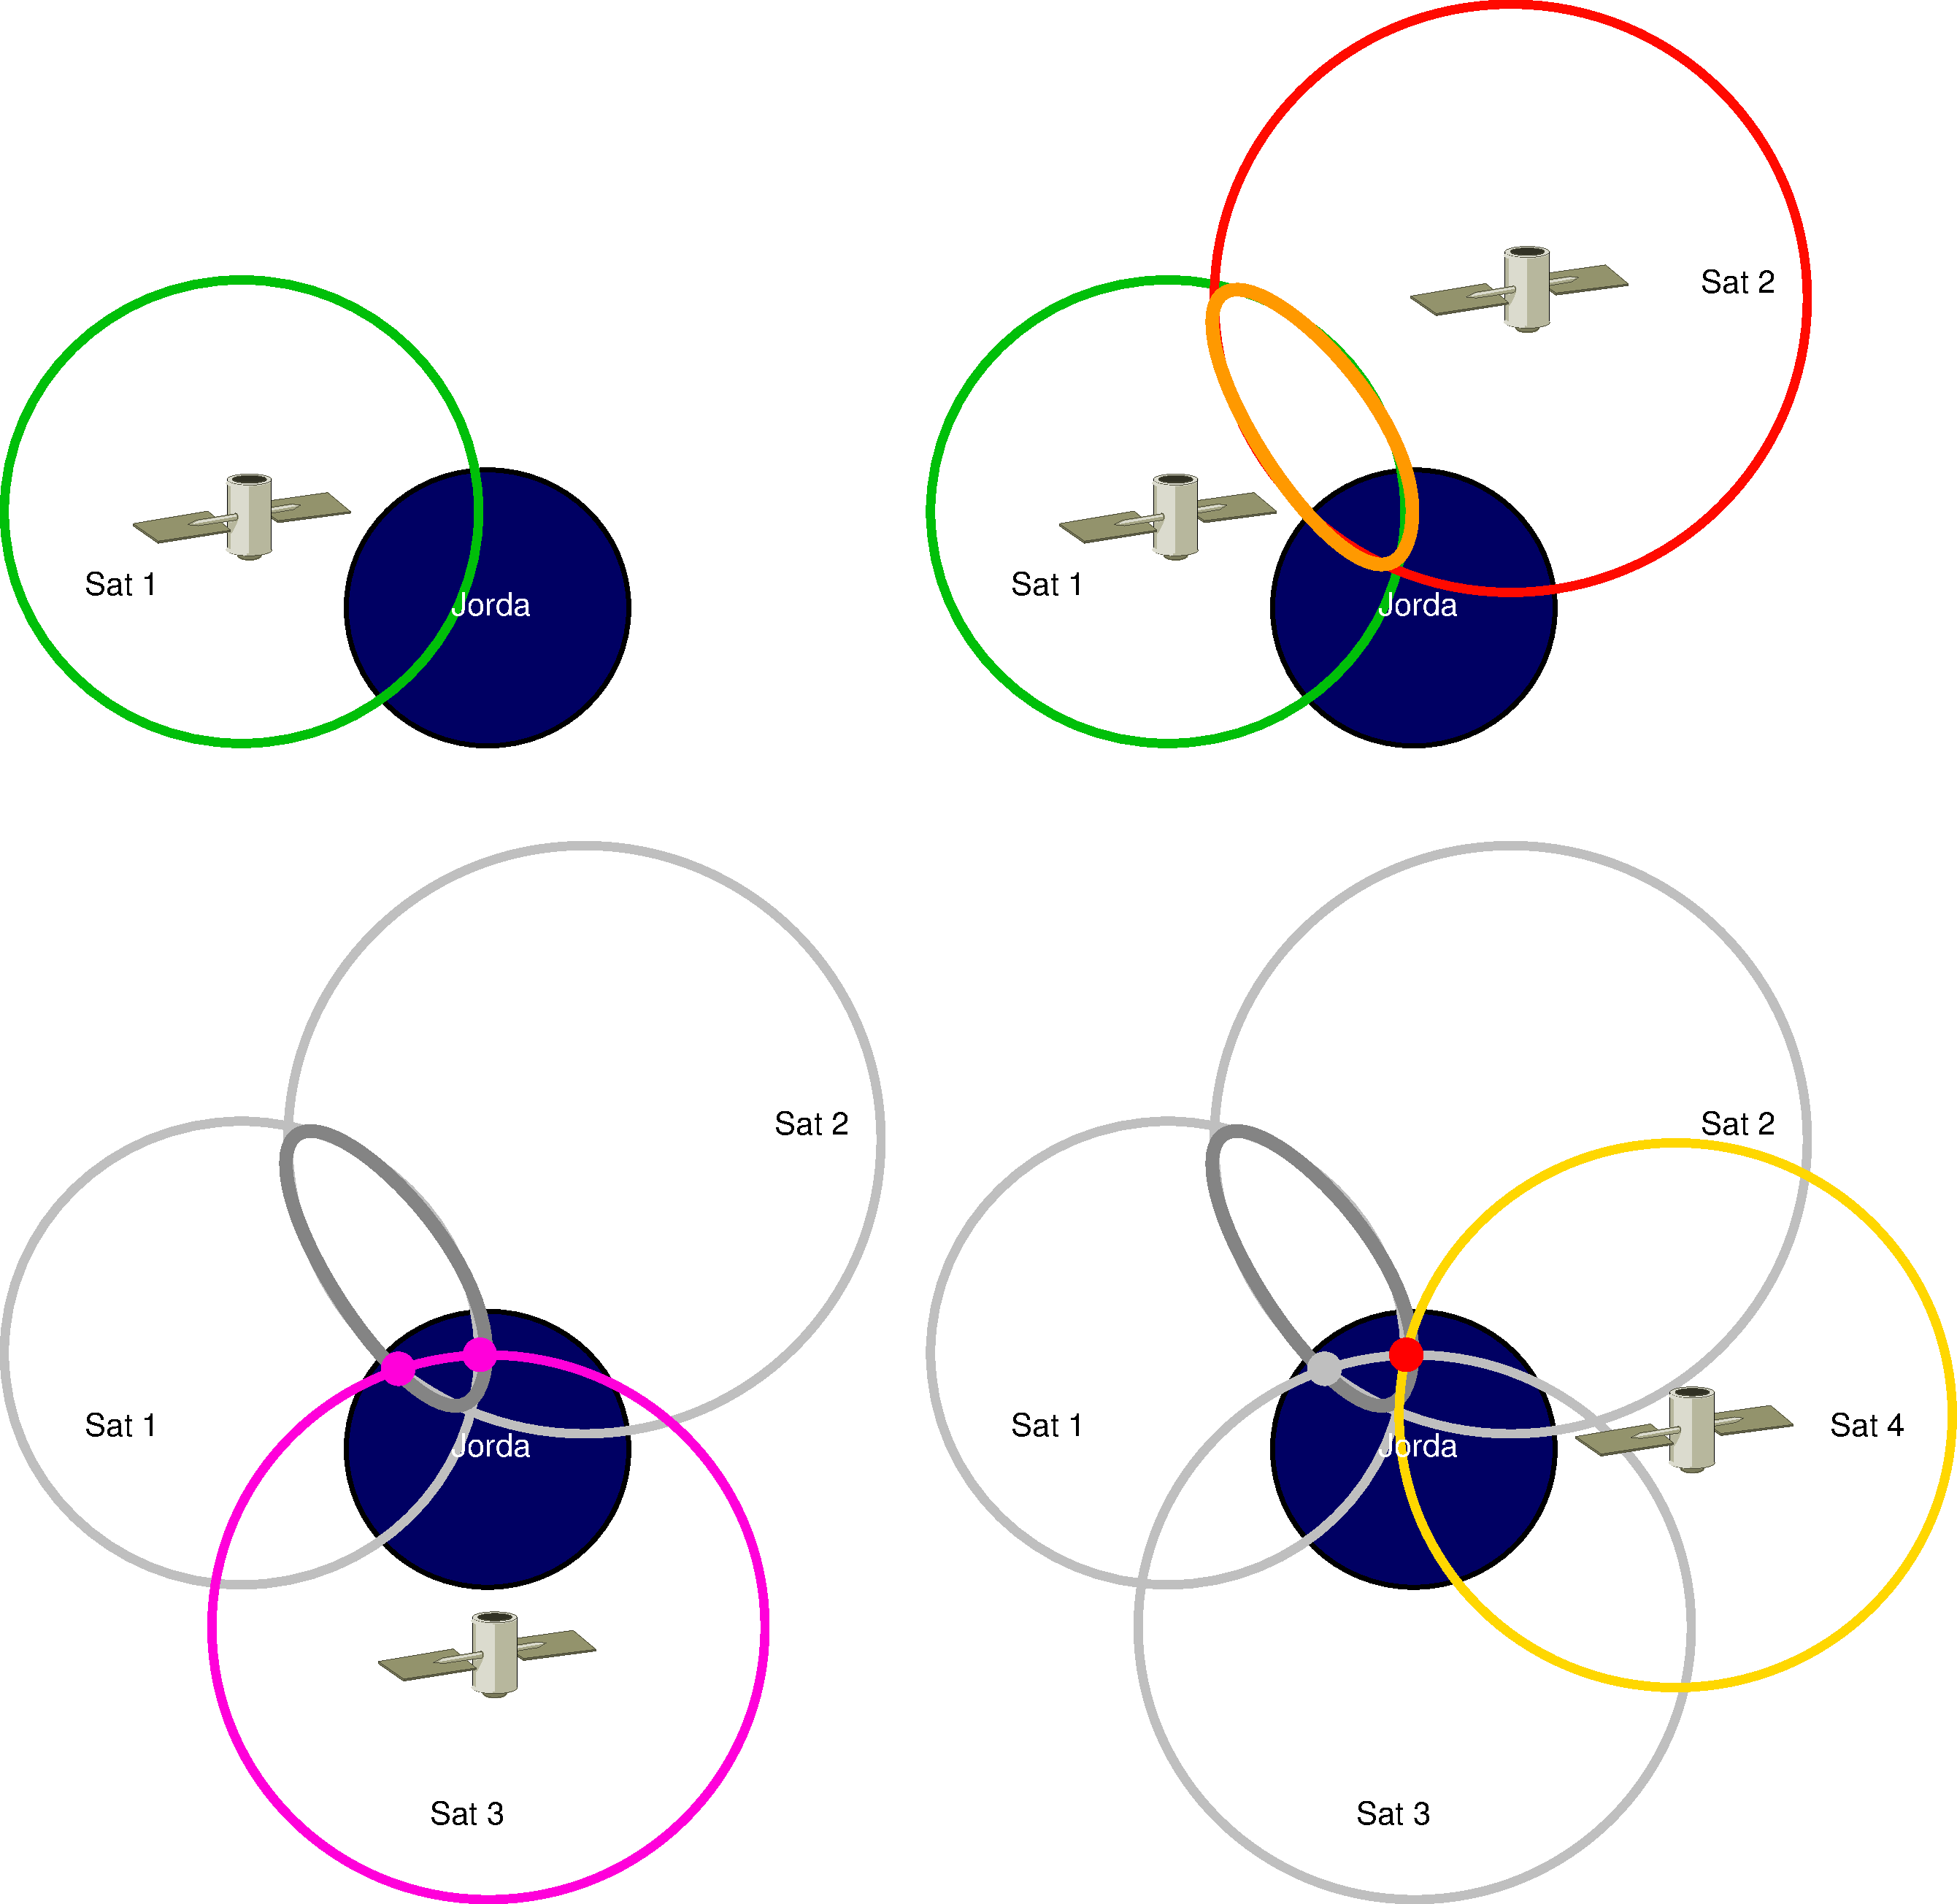
\includegraphics[scale=0.15]{thesis/graphics/trilaterate.pdf}
      \caption{Trilaterasjon}
      1 millisekund feil i klokka = 300 km feil i posisjon.
    \end{figure}
\end{frame}

\subsection{Anvendelse}
\begin{frame}
  \frametitle{Introduksjon}
\framesubtitle{GPS timing: Anvendelse}
  \begin{columns}
    \column{0.3\textwidth}
          \hspace{-50pt}
      \begin{figure}
        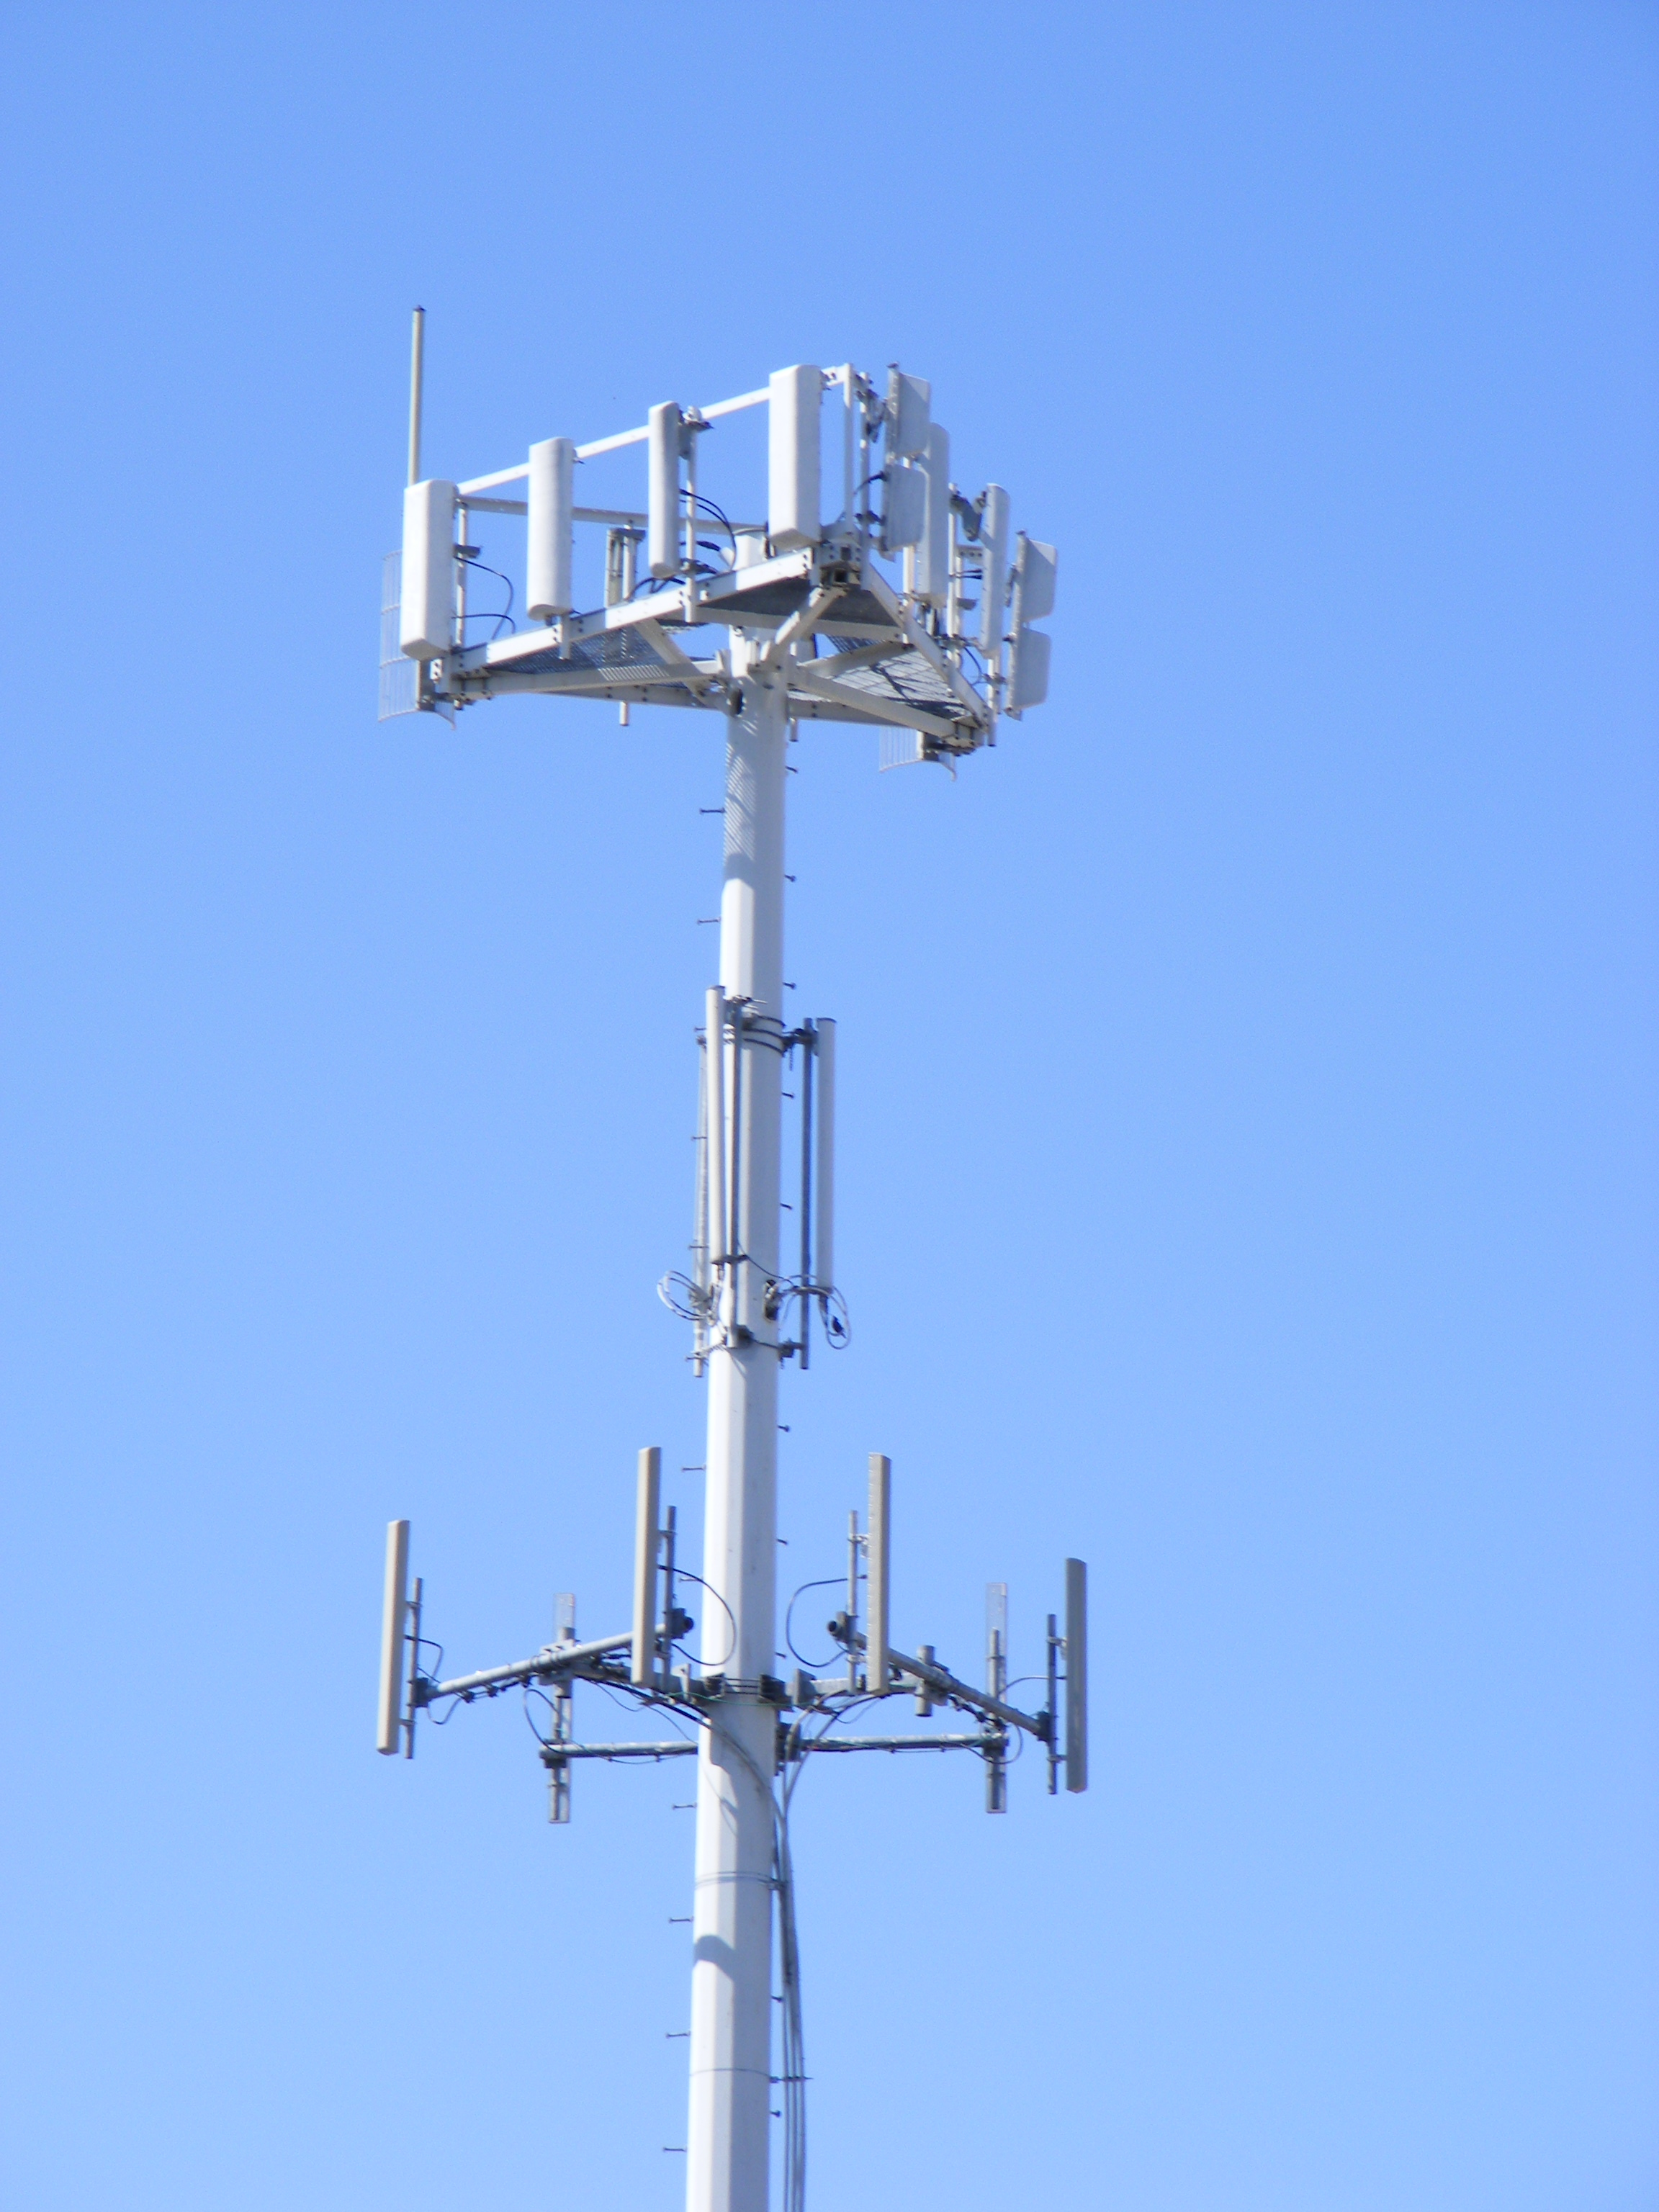
\includegraphics[scale=0.045]{thesis/graphics/Cell-Tower.jpg}
        \caption{Mobilmast \cite{CELLTOWER}}
      \end{figure}

    \column{0.3\textwidth}
              \hspace{-50pt}
      \begin{figure}
        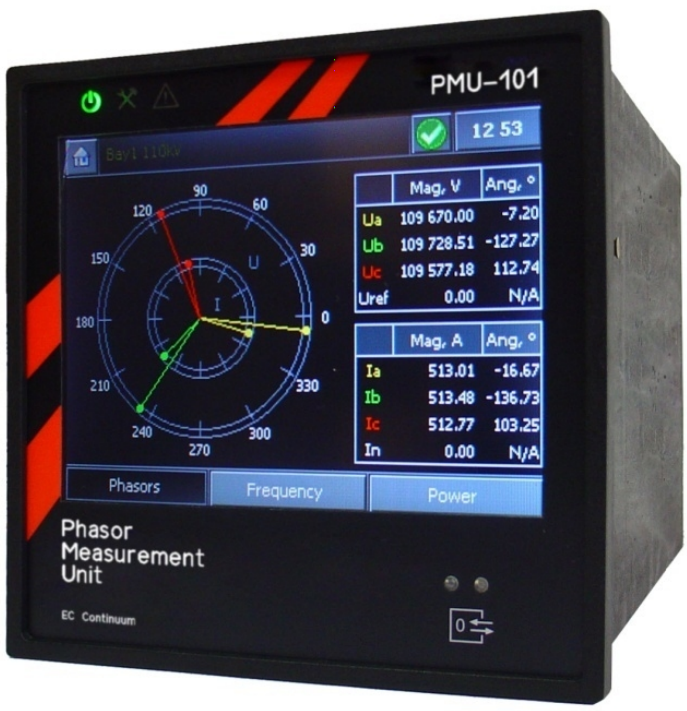
\includegraphics[scale=0.1]{thesis/graphics/pmu.png}
        \caption{PMU \cite{PMU}}
      \end{figure}
    %\begin{itemize}
    %    \item Tidsstempling 
    %    \item Fasemålinger i kraftnett.
    %    \item Telekommunikasjon.
    %\end{itemize}
    \column{0.3\textwidth}
              \hspace{-100pt}
    \begin{figure}
        \includegraphics[scale=0.025]{thesis/graphics/New_York_Stock_Exchange,_Wall_Street.jpg}
        \caption{Wall Street \cite{NEWYORK}}
      \end{figure}
  \end{columns}
\end{frame}

\subsection{Utfordringer og trusler}
\begin{frame}
  \frametitle{Introduksjon}
\framesubtitle{Utfordringer og trusler}
  Utfordringer:
  \begin{itemize}
    \item Avhengig av å ha en antenne med fri sikt.
    \item Kjent kodestruktur.
    \item Naive mottakere.
  \end{itemize}
  Trusler:
  \begin{itemize}
    \item Jamming.
    \item Spoofing
    \item Feil i utstyr.
  \end{itemize} 
\end{frame}

\begin{frame}
  \frametitle{Introduksjon}
\framesubtitle{Utfordringer og trusler}
      \begin{figure}
        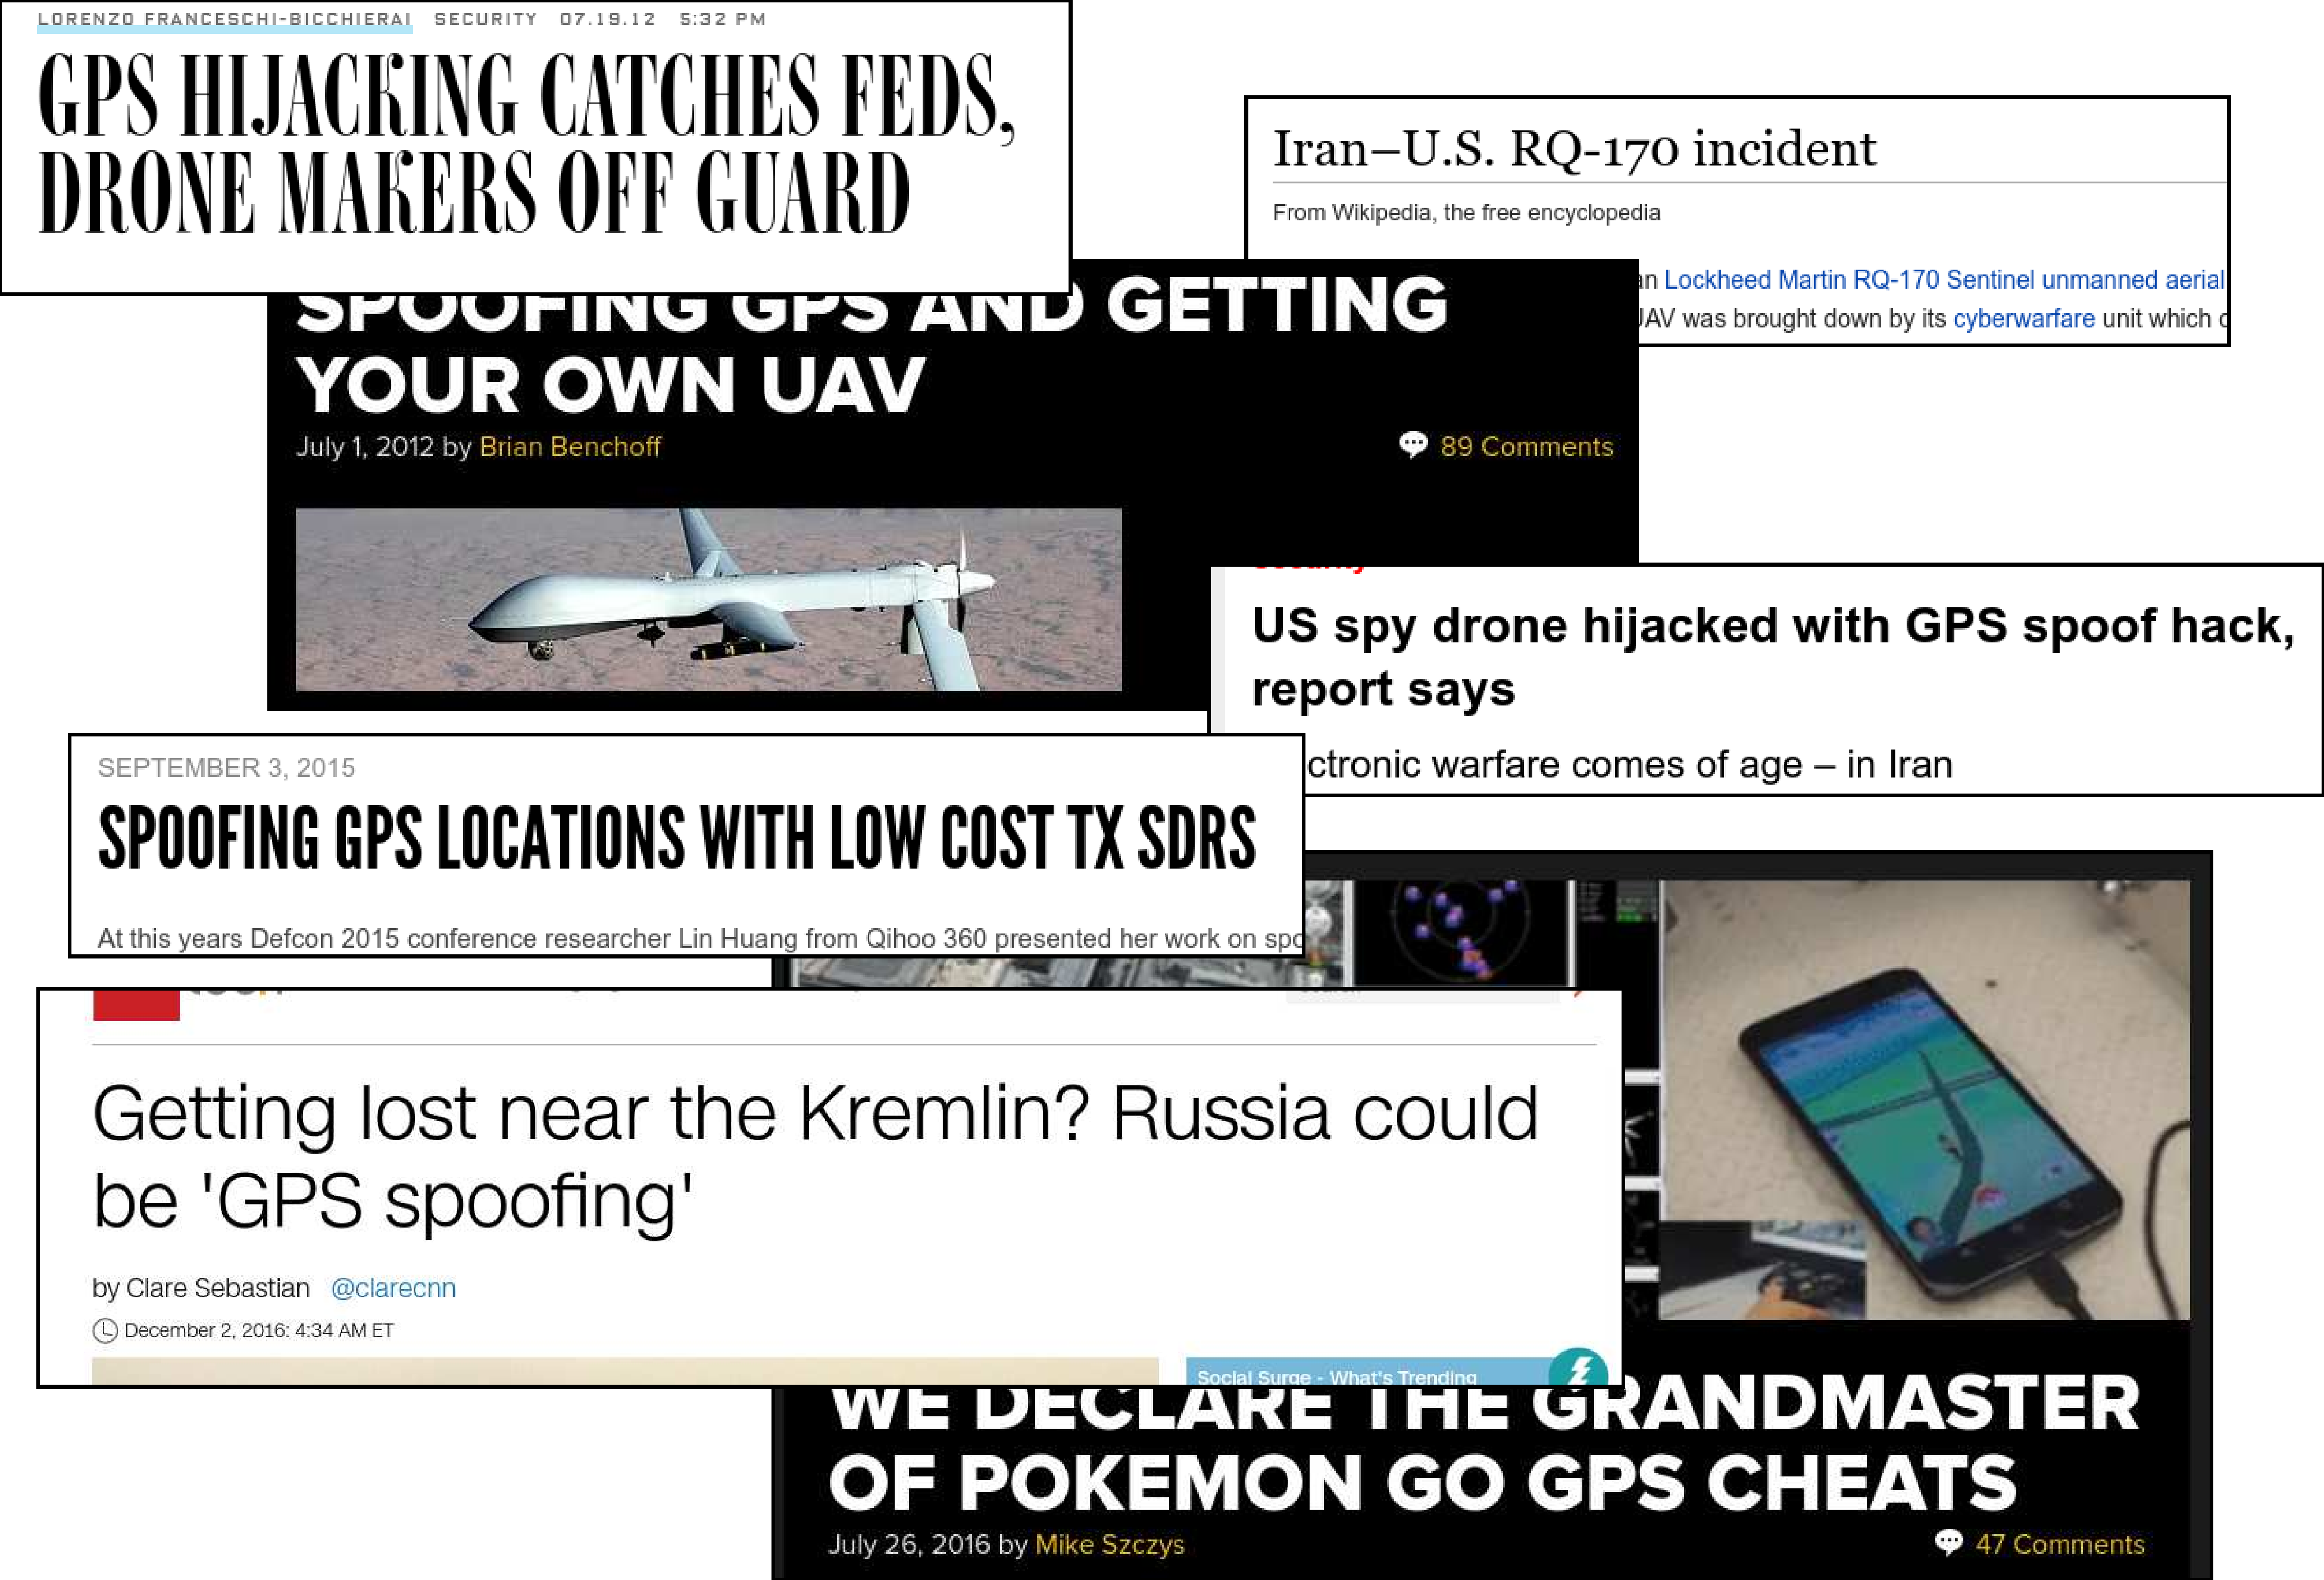
\includegraphics[scale=0.15]{thesis/graphics/montage.pdf}
      \end{figure} 
\end{frame}

\begin{frame}
  \frametitle{Introduksjon}
\framesubtitle{Utfordringer og trusler}
      \begin{figure}
        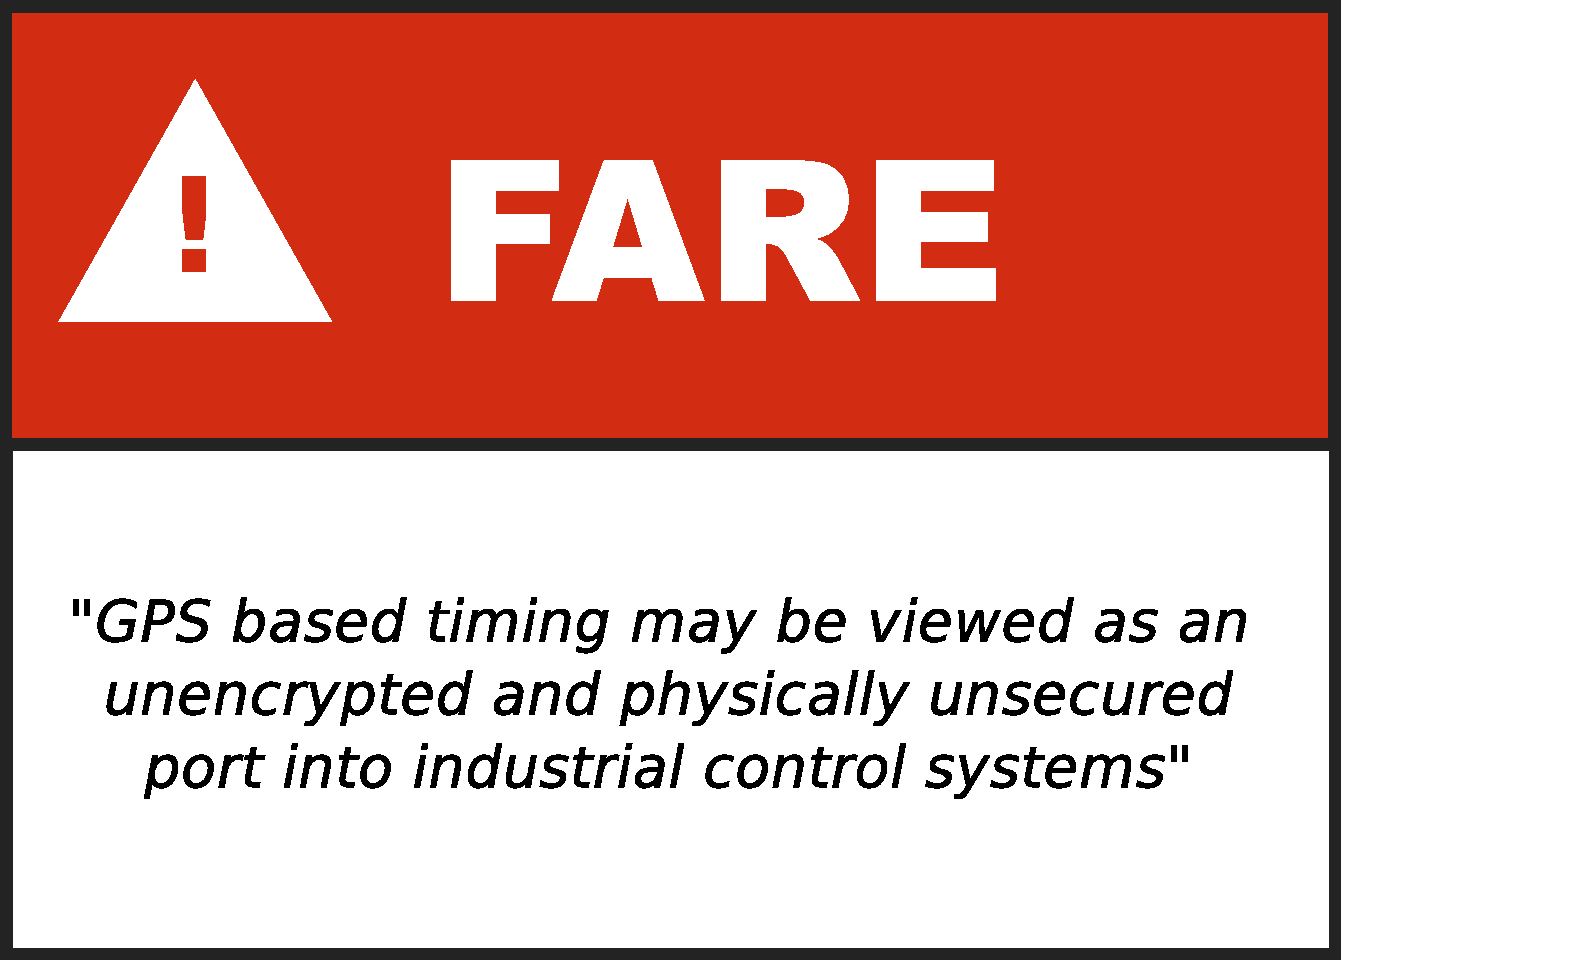
\includegraphics[scale=0.40]{thesis/graphics/fare.pdf}
      \end{figure} 
\end{frame}

\subsubsection{Referansetrusselen}
\begin{frame}
  \frametitle{Introduksjon}
  \framesubtitle{Referansetrusselen}
  \begin{figure}
    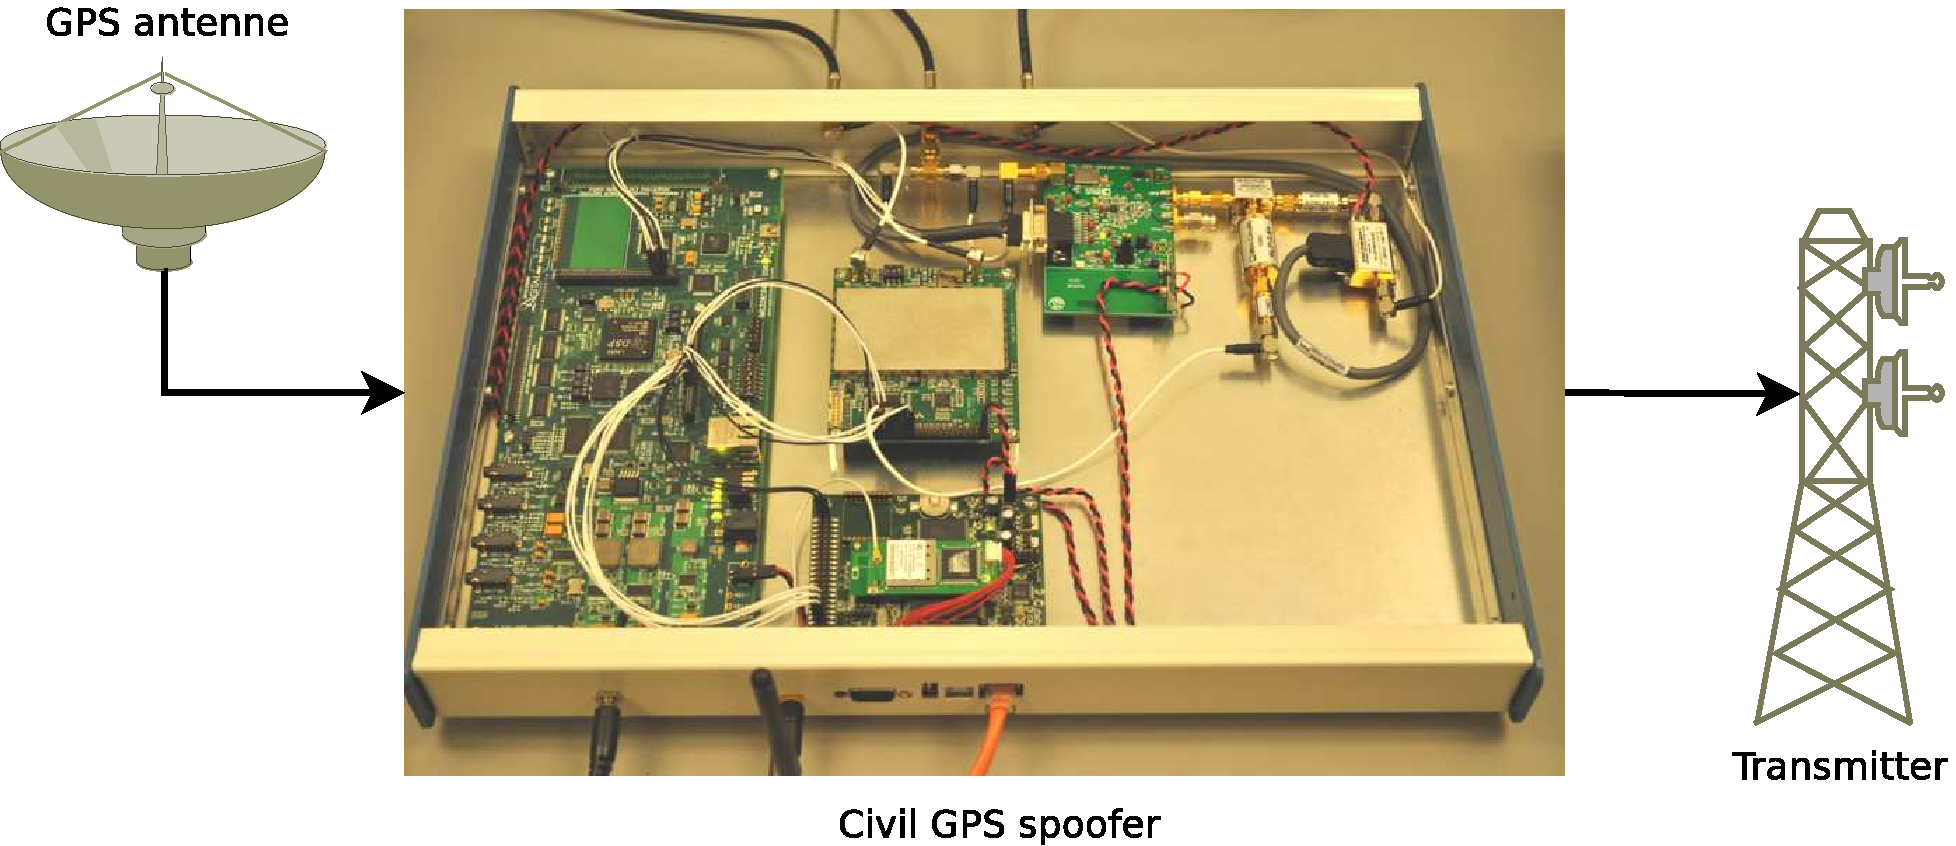
\includegraphics[scale=0.2]{thesis/graphics/spoofer_diagram.pdf}
    \caption{Civil GPS Spoofer \cite{EVPMUGA}}
  \end{figure}
  \begin{itemize}
  \item Laget et av et team fra \textit{The University of Texas at Austin} i 2012
  \item Software-definert radio
  \item 14 «falske» satellitter
  \item Sømløs narring
  \end{itemize}
\end{frame}

%\begin{frame}
%  \frametitle{"The Civil GPS Spoofer"}
%  Nøkkelfunksjoner:
%  \begin{itemize}
%    \item Sømløs narring, offeret låser på en kopi av det autentiske signalet. Ingen forandring i løsning.
%    \item Angriper manipulerer signalet.
%    \item Angriperen har gjerne et stort spillerom under angrepet da oscillatoren i mottakeren ofte er av lav kvalitet.
%  \end{itemize}
%\end{frame}

\section{Deteksjon og mottiltak}
\begin{frame}
\frametitle{Deteksjon og mottiltak}
  \begin{itemize}
        \setlength\itemsep{1em}
      \item Sammenlikne kjent posisjon mot løst.
      \item Bruke flere GPS-mottakere.
      \item Bruke god klokke for vurdering av tidsløsning.
        \begin{itemize}
          \item Også mottiltak!
        \end{itemize}
    \end{itemize}
\end{frame}

\subsection{Flere GPS mottakere}
\begin{frame} 
\frametitle{Deteksjon og mottiltak}
  \framesubtitle{Flere GPS mottakere og kjent posisjon}
  \begin{figure}
    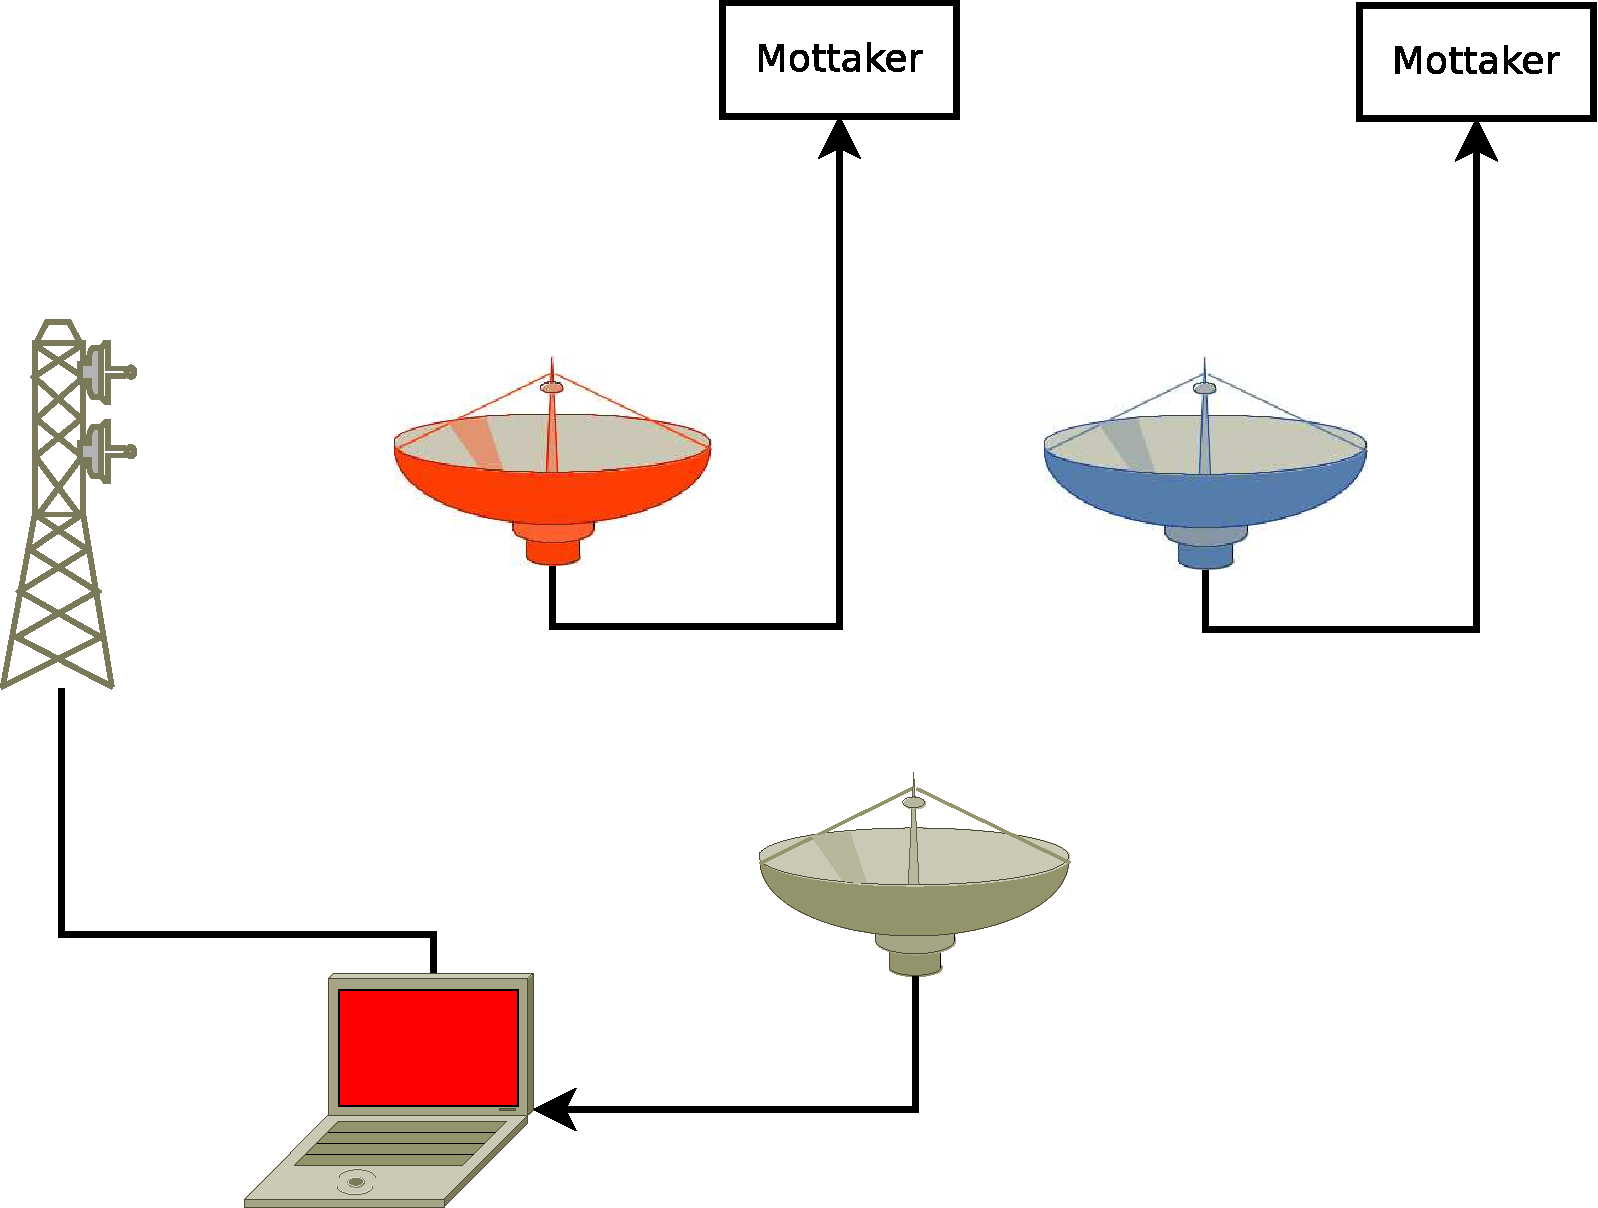
\includegraphics[scale=0.23]{thesis/graphics/toantenner.pdf}
    \caption{Spoofing deteksjon med to antenner}
  \end{figure}
\end{frame}

\begin{frame} 
\frametitle{Deteksjon og mottiltak}
  \framesubtitle{Flere GPS mottakere og kjent posisjon}
  \begin{figure}
    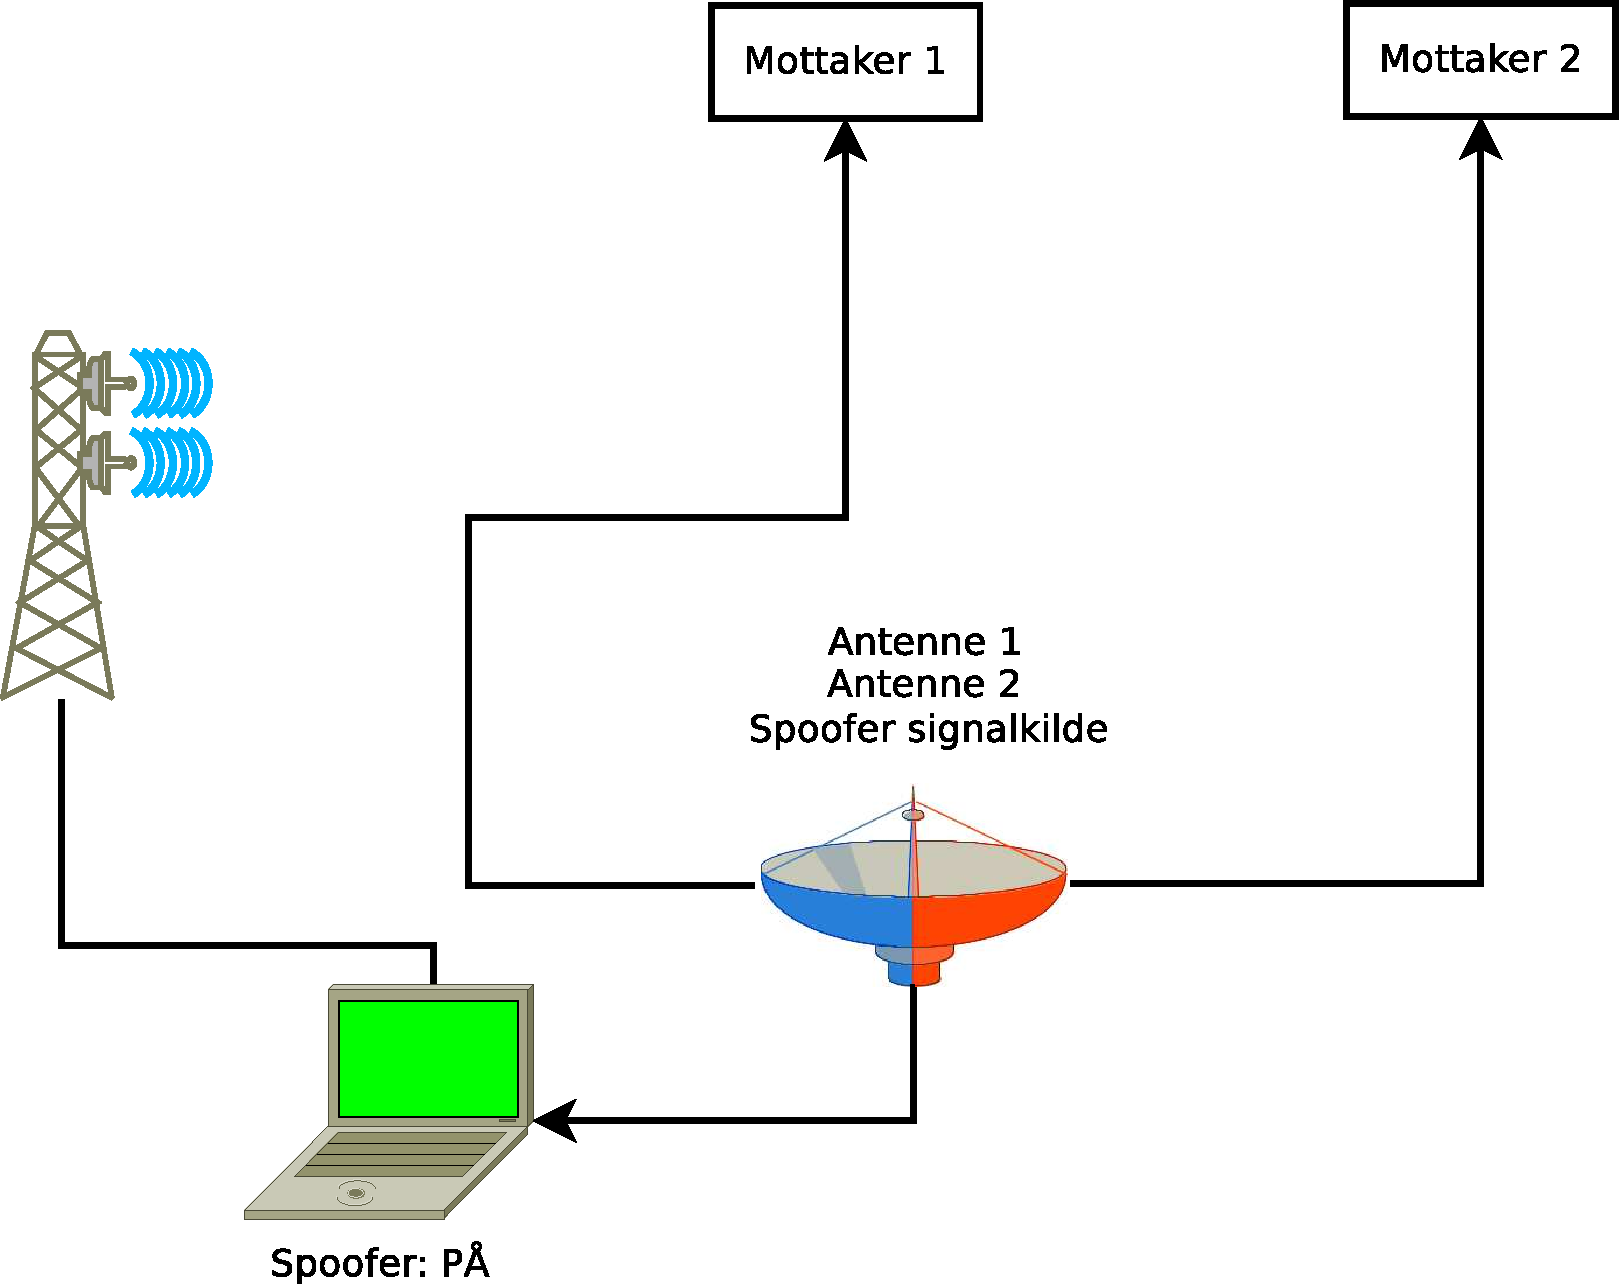
\includegraphics[scale=0.23]{thesis/graphics/toantenner_2.pdf}
    \caption{Spoofing deteksjon med to antenner}
  \end{figure}
\end{frame}

\subsection{En god klokke}
\begin{frame}
\frametitle{Deteksjon og mottiltak}
  \framesubtitle{En god klokke}
  \begin{columns}
    \column{0.5\textwidth}
    \begin{itemize}
          \setlength\itemsep{2em}
      \item Trenger få korreksjoner
      \item Lite påvirket av temperatur
      \item Intern frekvensteller og styringsalgoritme
    \end{itemize}
    \column{0.5\textwidth}
      \begin{figure}
        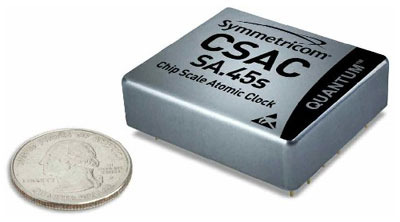
\includegraphics[scale=0.2]{thesis/graphics/csac.jpg}
      \caption{Symmetricom SA.45s CSAC \cite{SADS}}
    \end{figure}
  \end{columns}
\end{frame}

\begin{frame}
\frametitle{Deteksjon og mottiltak}
  \framesubtitle{En god klokke}
      \begin{figure}
        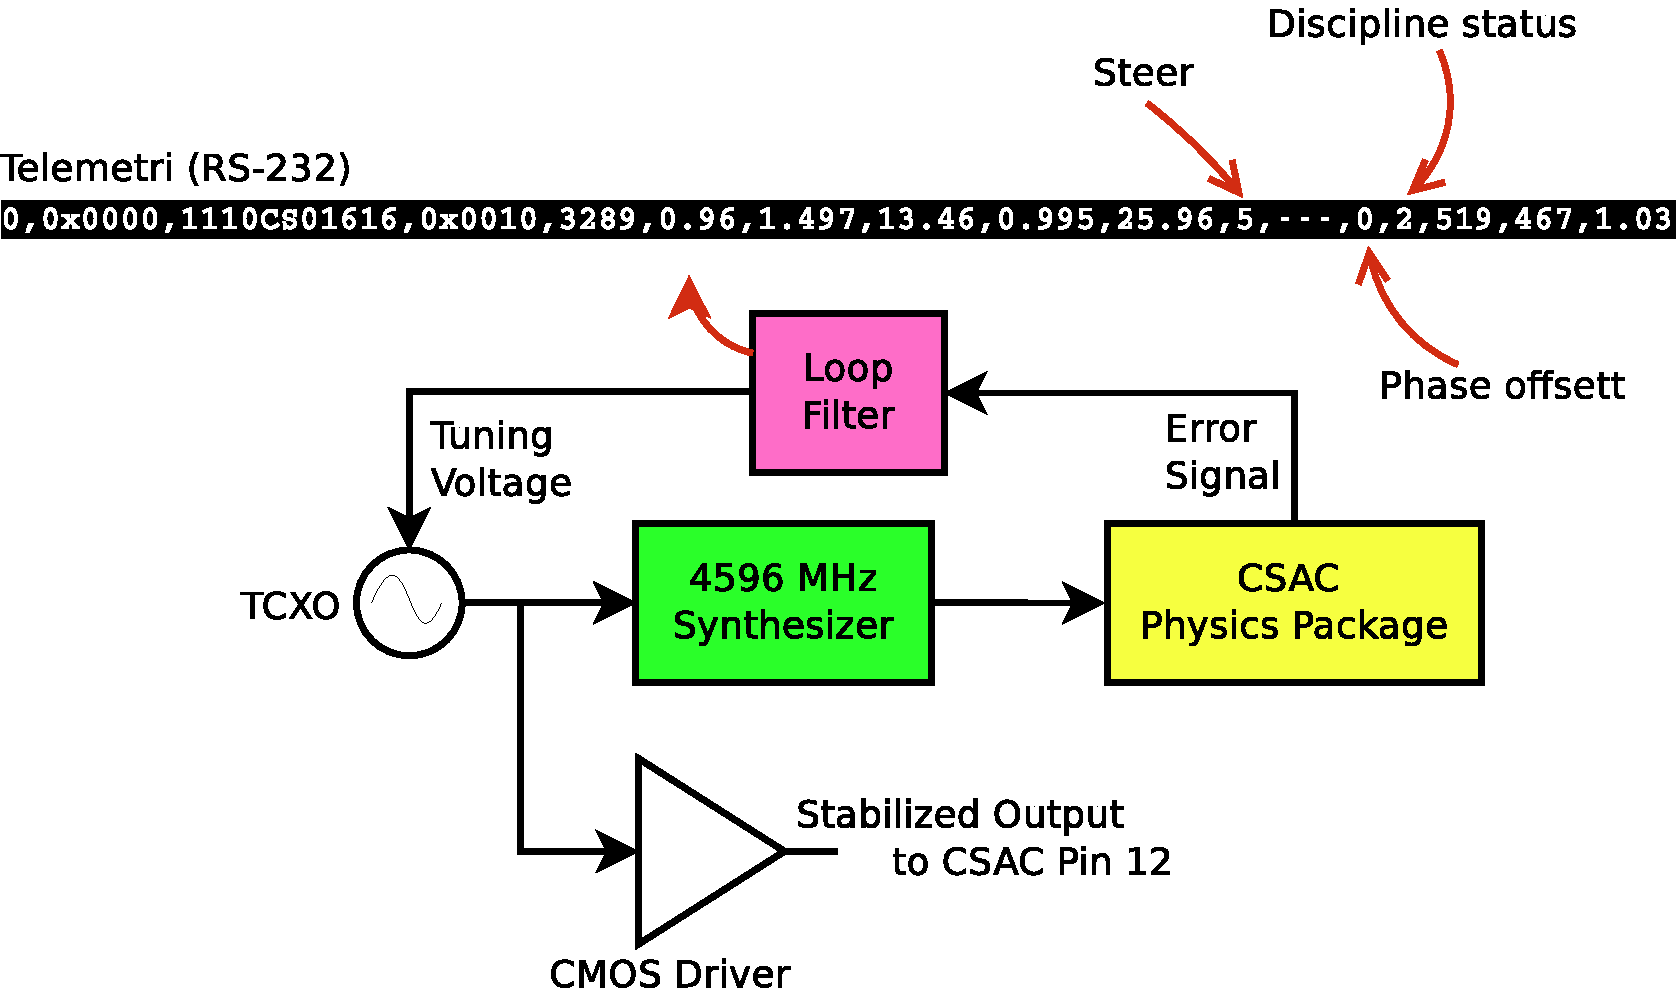
\includegraphics[scale=0.35]{thesis/graphics/csac_schematic.pdf}
      \caption{CSAC blokkdiagram}
    \end{figure}
\end{frame}

\section{System implementasjon}
\subsection{Ønsket funksjonalitet}
\begin{frame}
\frametitle{Systemimplementasjon}
  \framesubtitle{Ønsket funksjonalitet}
  \begin{itemize}
    \item Detektere angrep
    \item Logging
    \item Enkel utbygging
    \item Administreres over nettverk
    \item Konfigurerbar 
  \end{itemize}
\end{frame}

\subsection{Klokkemodell}
\begin{frame}
\frametitle{Systemimplementasjon}
  \framesubtitle{Klokkemodell}
  \begin{itemize}
    \item Utviklet av Harald Hauglin
    \item Bruker klokkedata (telemetri)
    \item $10^{-11}$ relativ frekvensfeil tilsvarer 1 mikrosekund/døgn
  \end{itemize}
    \begin{figure}
        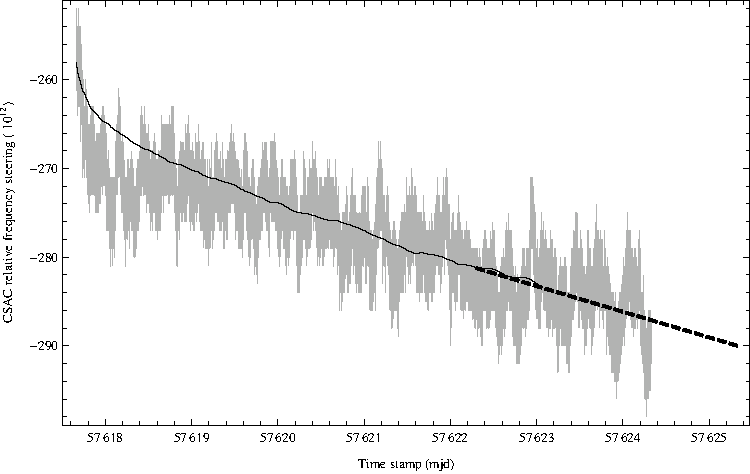
\includegraphics[scale=0.5]{thesis/graphics/csac_modelling_prediction.pdf}
      \caption{CSAC styringskorreksjon, fra klokke og predikert.}
    \end{figure}
    %Klokkemodellen brukt i oppgaven er designet av Harald Hauglin. Brukes til:
    %\begin{itemize}
    %  \item Referanse for frekvensavvik og klokkedrift 
    %  \item Generere brukbare styringsparameter i tilfelle GPS løsning ikke lenger er til å stole på.
    %\end{itemize}
    %Modellen er logisk en del av serveren og kjører i en egen prosess.
    %\begin{itemize}
    %  \item Kommuniserer med atomklokka
    %  \item Moden etter to dager (konfigurerbart).
    %\end{itemize}
\end{frame}

\subsection{Filtre}
\begin{frame}
\frametitle{Systemimplementasjon}
  \framesubtitle{Filtre}
  \begin{itemize}
        \setlength\itemsep{2em}
    \item Sted og hastighet (GPS)
                  %\begin{itemize}
                  %  \item Data fra sensorene blir samlet formatert.
                  %  \item Sjekker løst posisjon og hastighet mot referanseverdier
                  %\end{itemize}
    \item Fasehopp (Klokke)
                   % \begin{itemize}
                   %   \item Sammenlikner nåværende fase med pre-konfigurert grense.
                   % \end{itemize}
    \item Frekvenskorreksjon (Klokke)
                   % \begin{itemize}
                   %   \item Sammenlikner nåværende styringsverdi med en forventet styringsverdi
                   % \end{itemize}
  \end{itemize}
  %Pre-konfigurerte referanseverdier er basert på et gjennomsnitt kalkulert fra en lengre måleserie.
\end{frame}

\subsection{Sensor Client/Server}
\begin{frame}
\frametitle{Systemimplementasjon}
  \framesubtitle{Sensor server: Idé}
    \begin{figure}
      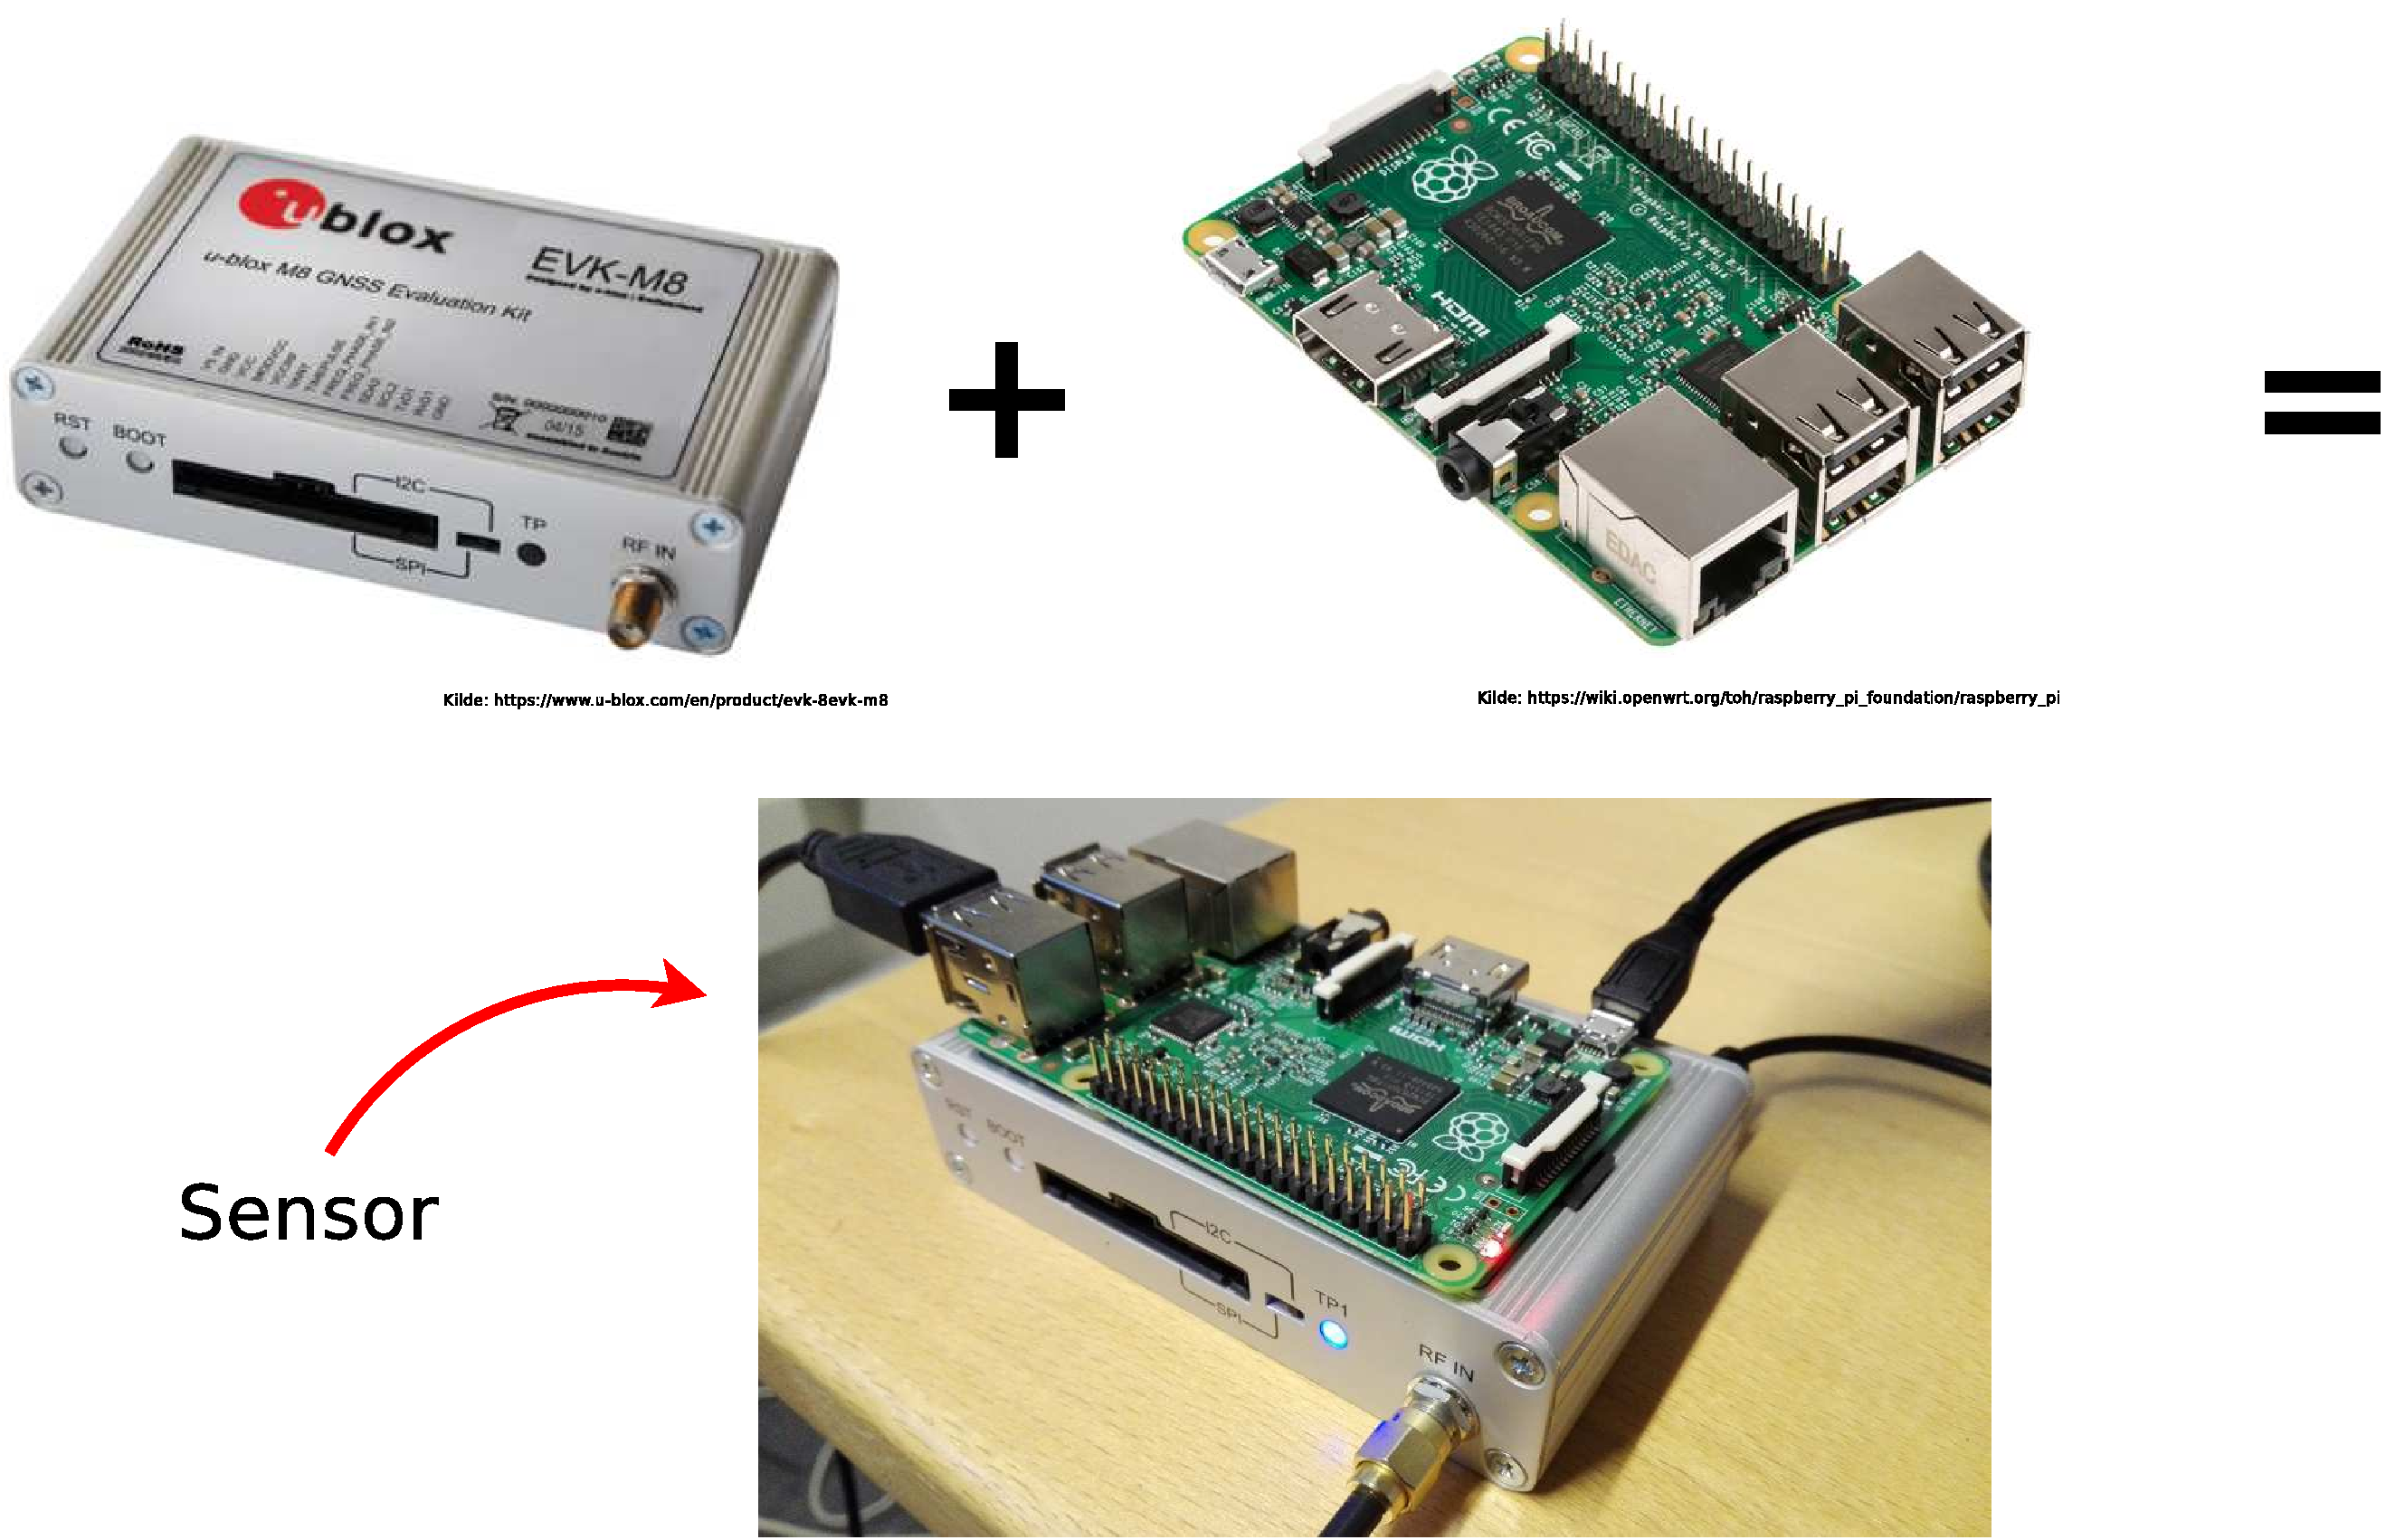
\includegraphics[scale=0.2]{thesis/graphics/raspi_gps.pdf}
    \end{figure}
  %\begin{itemize}
  %  \item Mottaker + Raspberry PI = Sensor
  %  \item Eliminerer behovet for lange signalkabler, bruke nettverk:
  %  \begin{itemize}
  %    \item Fiber
  %    \item Mobilnett (3G og 4G)
  %    \item WiFi
  %  \end{itemize}
  %  \item Antall mottakere begrenset av serverens maskinvare.
  %\end{itemize}
\end{frame}

\begin{frame}
\frametitle{Systemimplementasjon}
  \framesubtitle{Sensor Client}
    \begin{figure}
      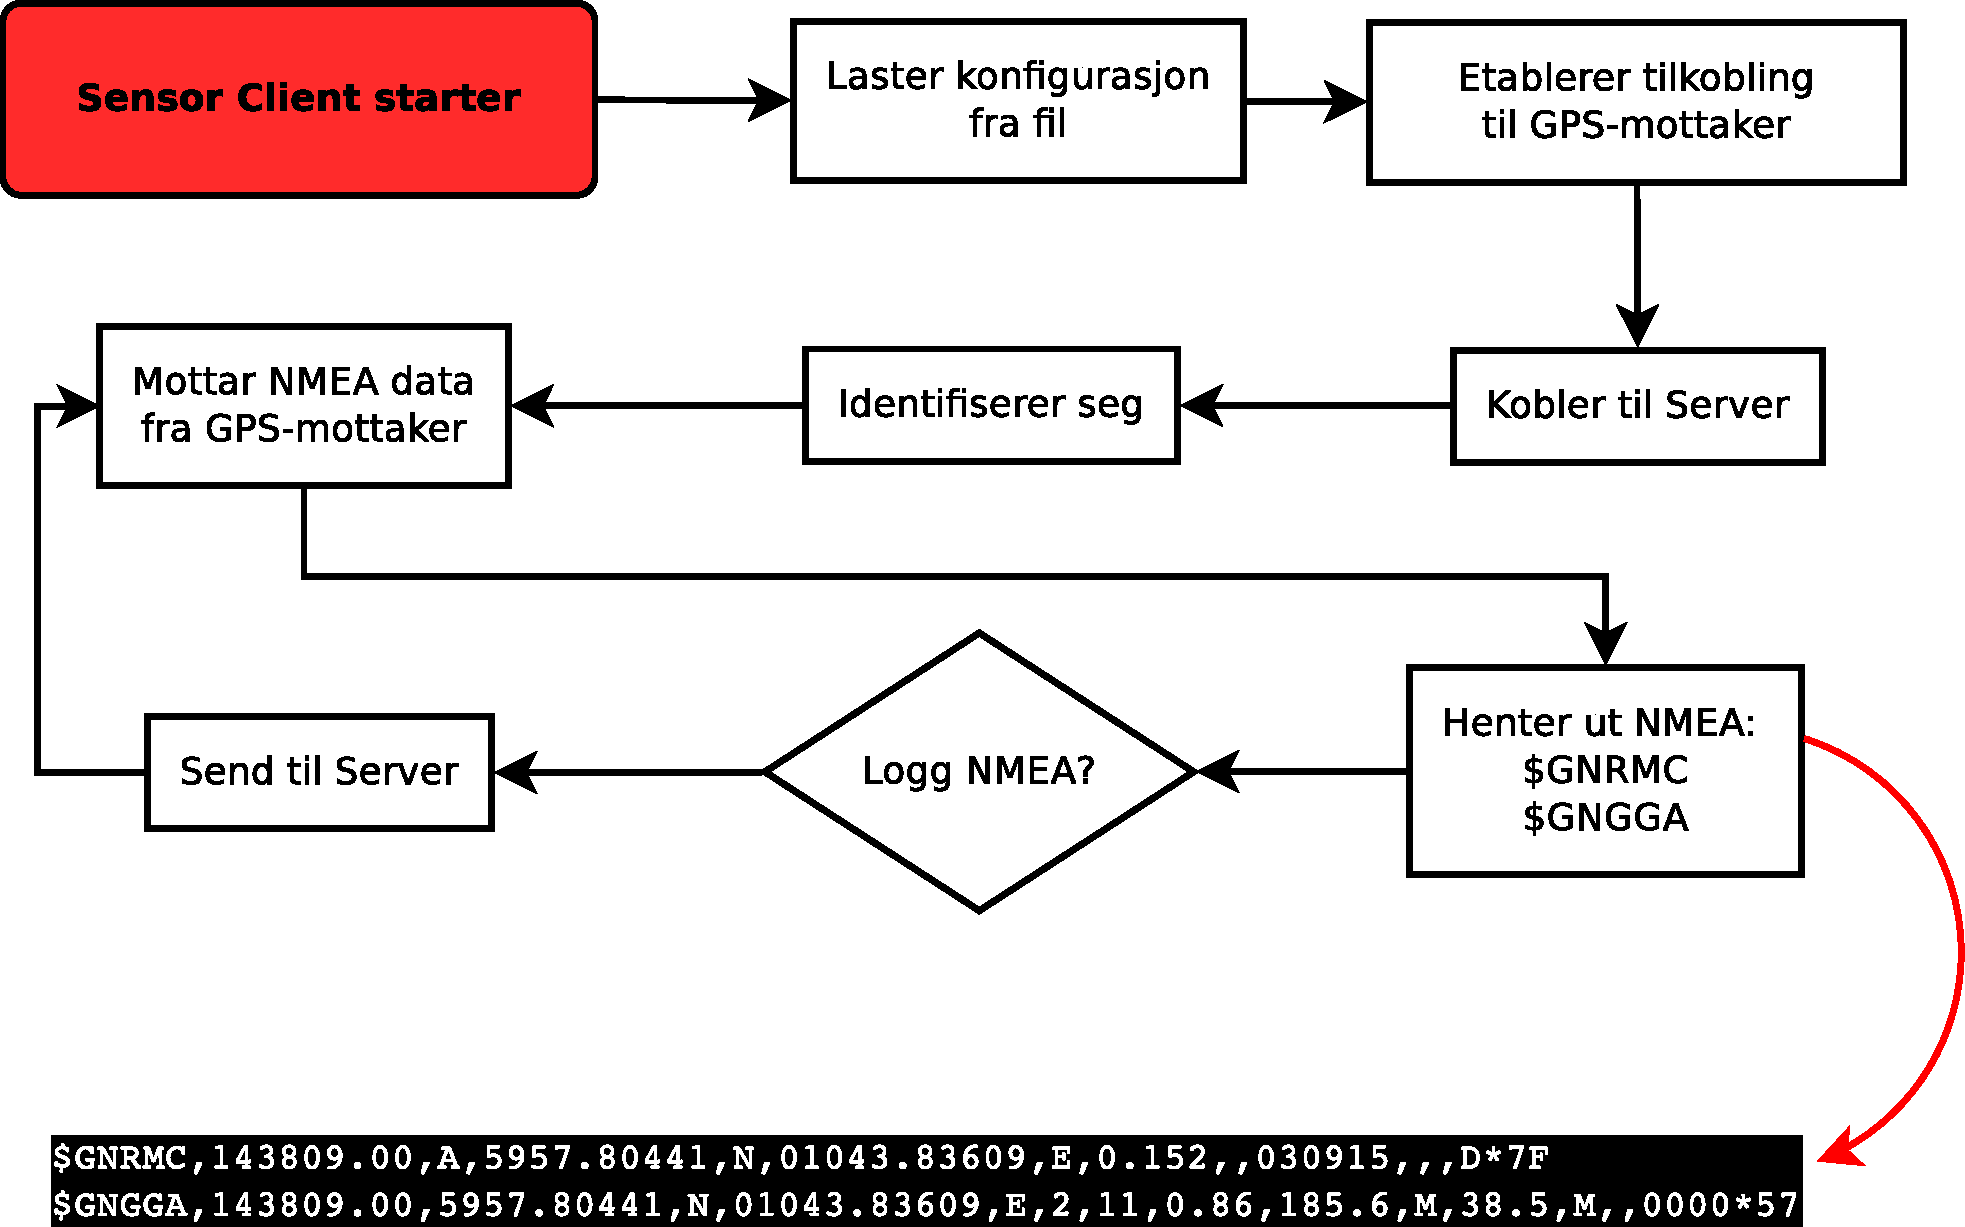
\includegraphics[scale=0.25]{thesis/graphics/client_simplified.pdf}
    \end{figure}
    %\item 3000+ linjer med C99 kode
    %\item Håndterer av/pålogging av klienter
    %\item Håndtere mottak og formatering av GPS data
    %\item En prosess per pålogging
    %\item Delt minne mellom prosesser (anonym MMAP)
    %  \begin{itemize}
    %    \item Semaforer og barrierer for beskyttelse
    %  \end{itemize}
    %\item Mulighet for brukere å koble på og gi kommandoer, f.eks:
    %  \begin{itemize}
    %    \item Rapporterer lokasjon og tid
    %    \item Rapportere server status
    %    \item Rapportere filterstatus
    %    \item Lagre og gjenopprette tilstand i sensorer
    %    \item Laste inn nye lokasjonsdata
    %    \item Avslutte egen og andres tilkobling
    %    \item Sende kommandoer til atomklokka 
    %  \end{itemize}
  %\end{itemize}
\end{frame}

\begin{frame}
\frametitle{Systemimplementasjon}
  \framesubtitle{Sensor server: Arkitektur}
    \begin{figure}
      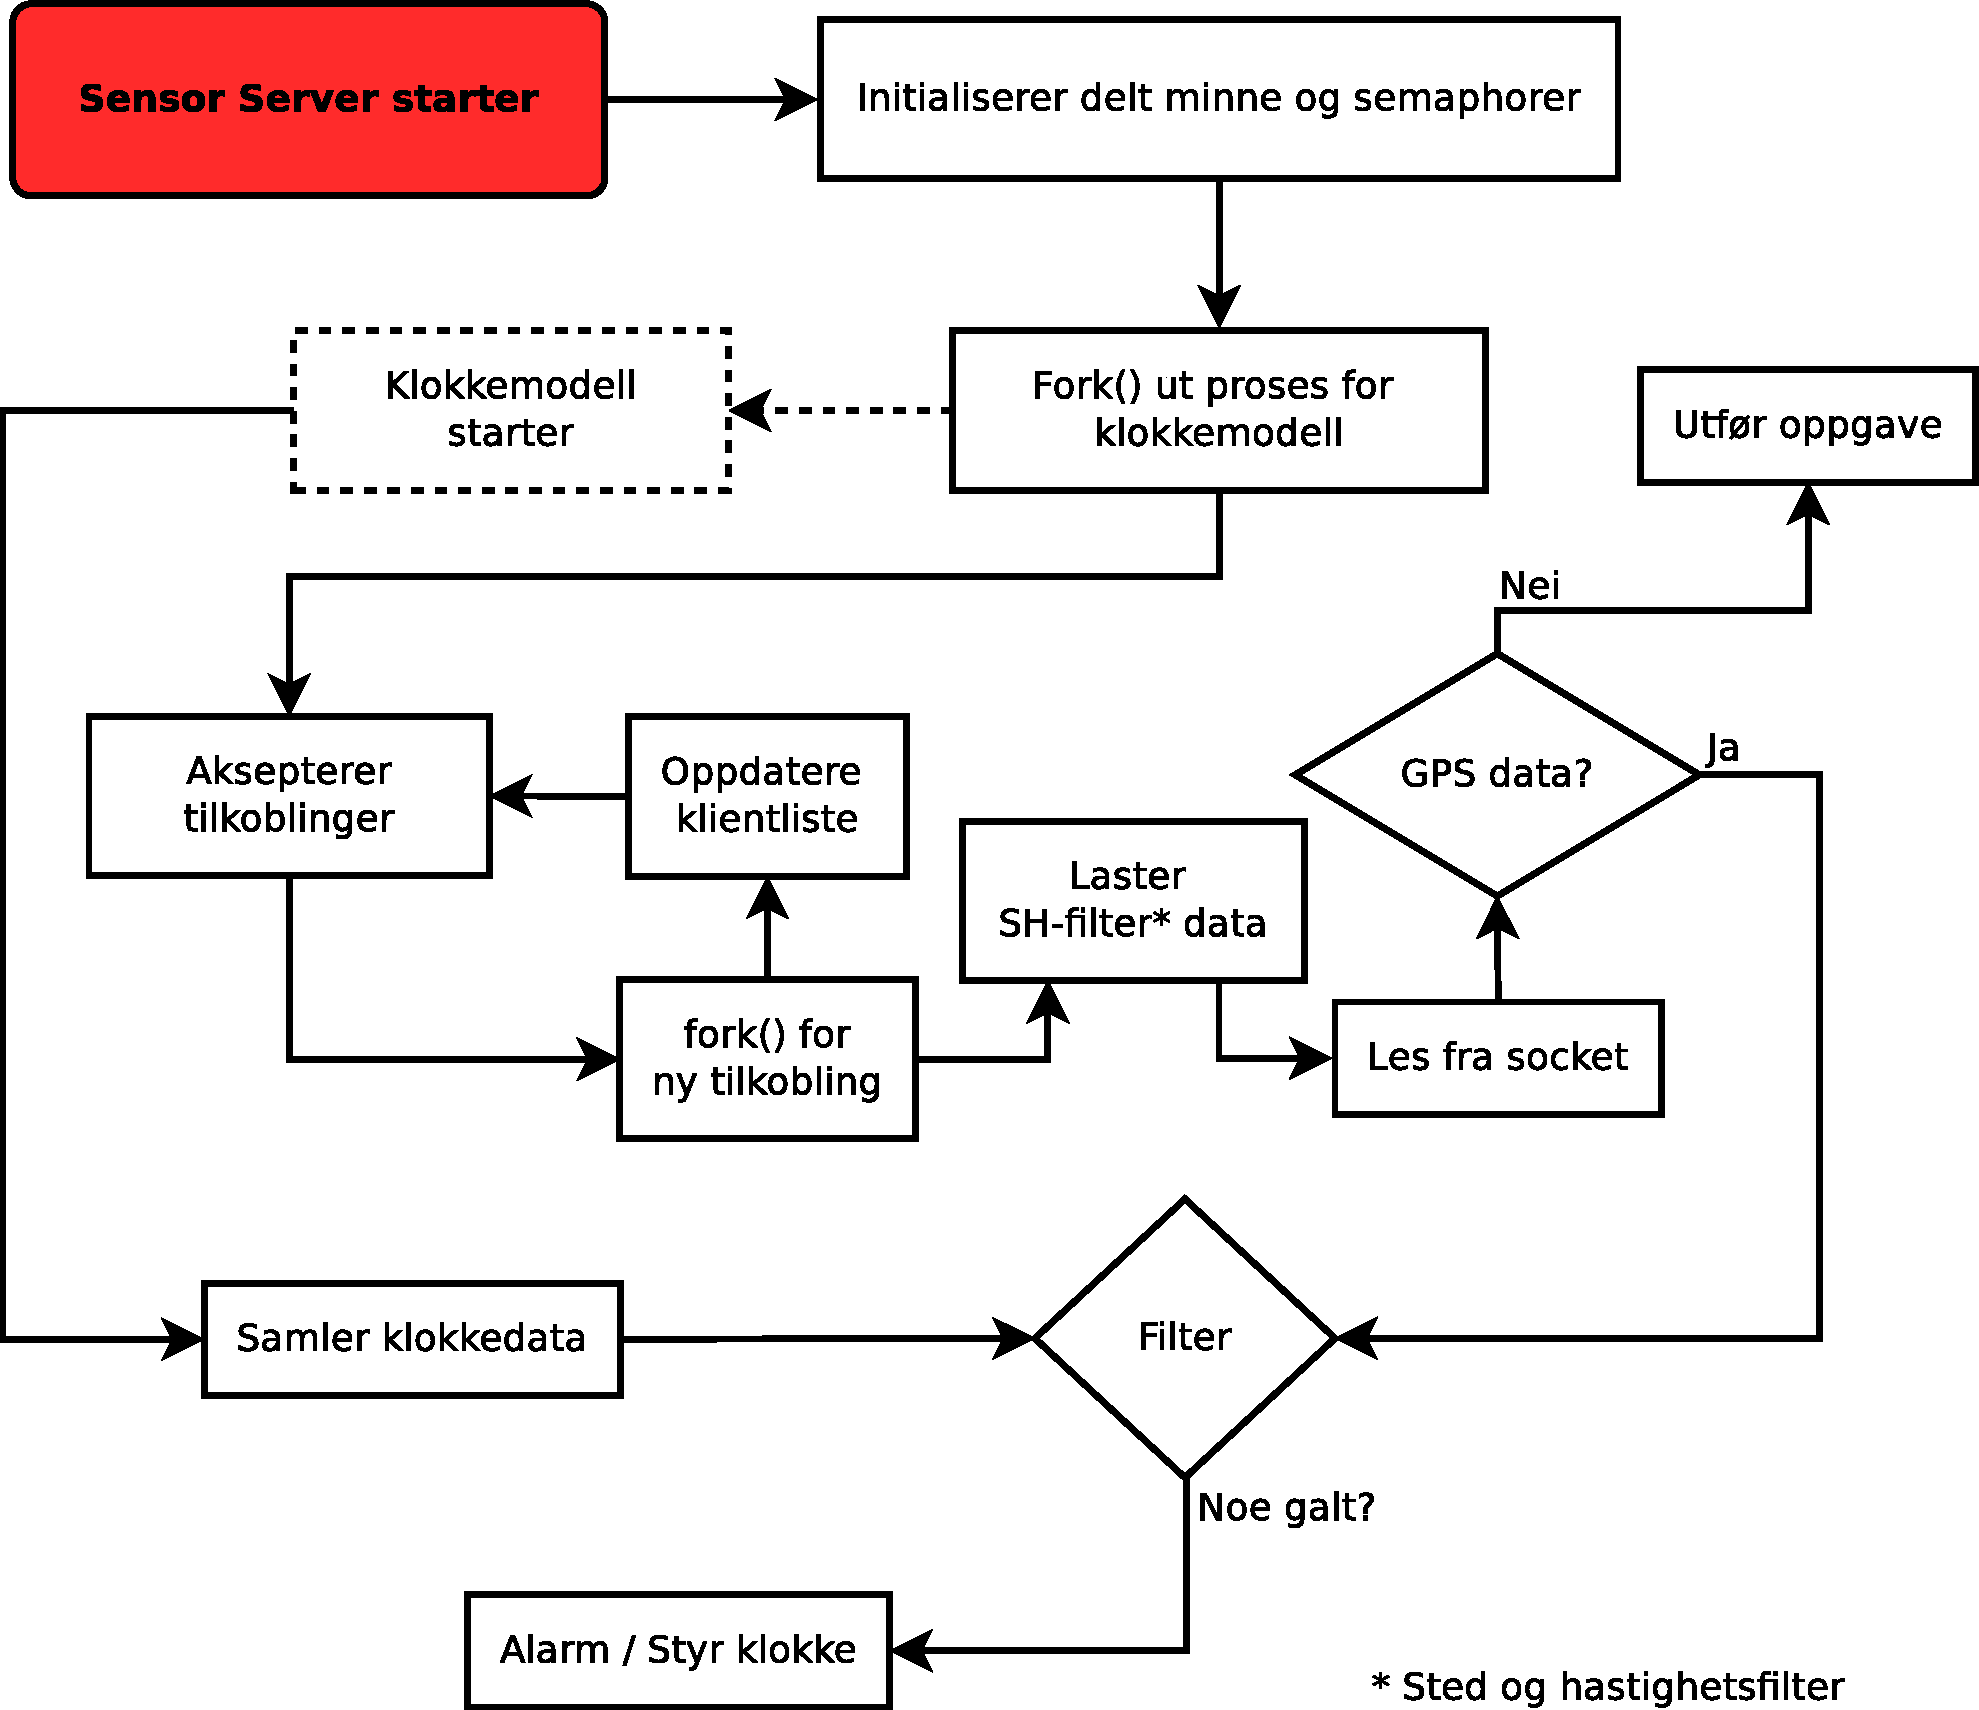
\includegraphics[scale=0.25]{thesis/graphics/csac_core_simplified.pdf}
    \end{figure}
    %\item 3000+ linjer med C99 kode
    %\item Håndterer av/pålogging av klienter
    %\item Håndtere mottak og formatering av GPS data
    %\item En prosess per pålogging
    %\item Delt minne mellom prosesser (anonym MMAP)
    %  \begin{itemize}
    %    \item Semaforer og barrierer for beskyttelse
    %  \end{itemize}
    %\item Mulighet for brukere å koble på og gi kommandoer, f.eks:
    %  \begin{itemize}
    %    \item Rapporterer lokasjon og tid
    %    \item Rapportere server status
    %    \item Rapportere filterstatus
    %    \item Lagre og gjenopprette tilstand i sensorer
    %    \item Laste inn nye lokasjonsdata
    %    \item Avslutte egen og andres tilkobling
    %    \item Sende kommandoer til atomklokka 
    %  \end{itemize}
  %\end{itemize}
\end{frame}

\begin{frame}
\frametitle{Systemimplementasjon}
  \framesubtitle{Kommunikasjon: Roller}
    \begin{figure}
      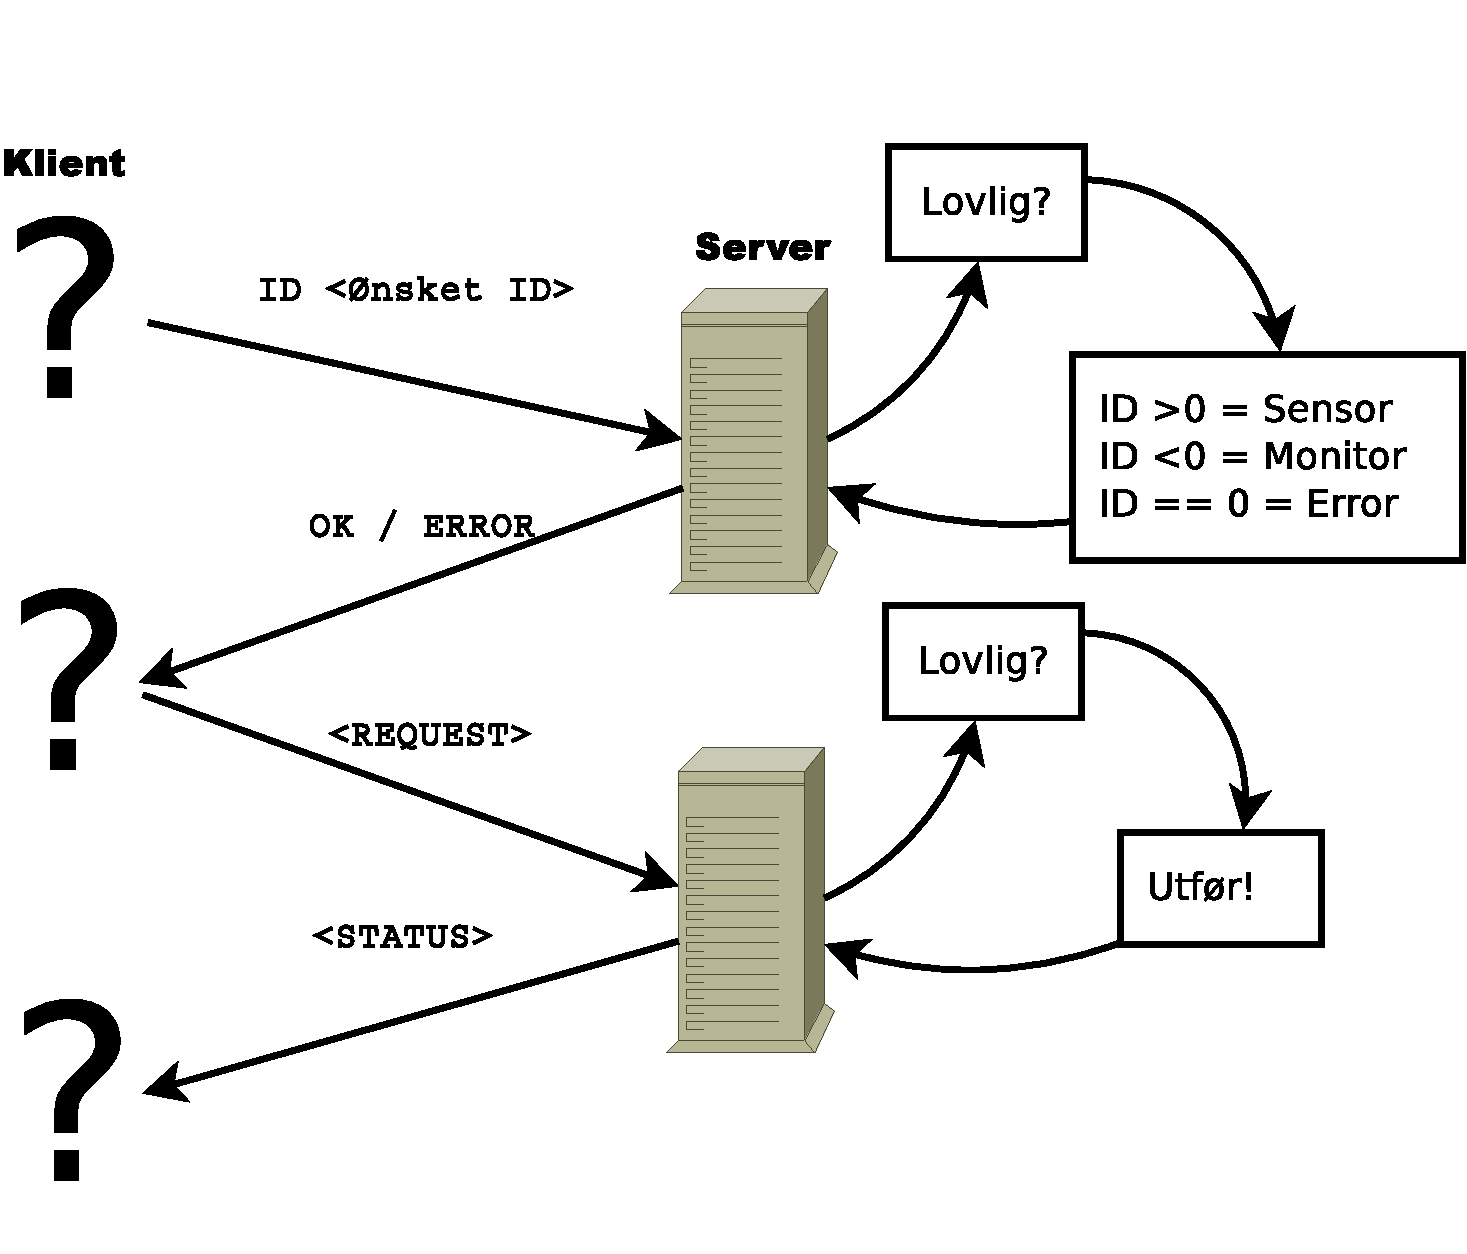
\includegraphics[scale=0.3]{thesis/graphics/server_explain.pdf}
    \end{figure}
\end{frame}

\begin{frame}
\frametitle{Systemimplementasjon}
  \framesubtitle{Kommunikasjon: GPS data}
    \begin{figure}
      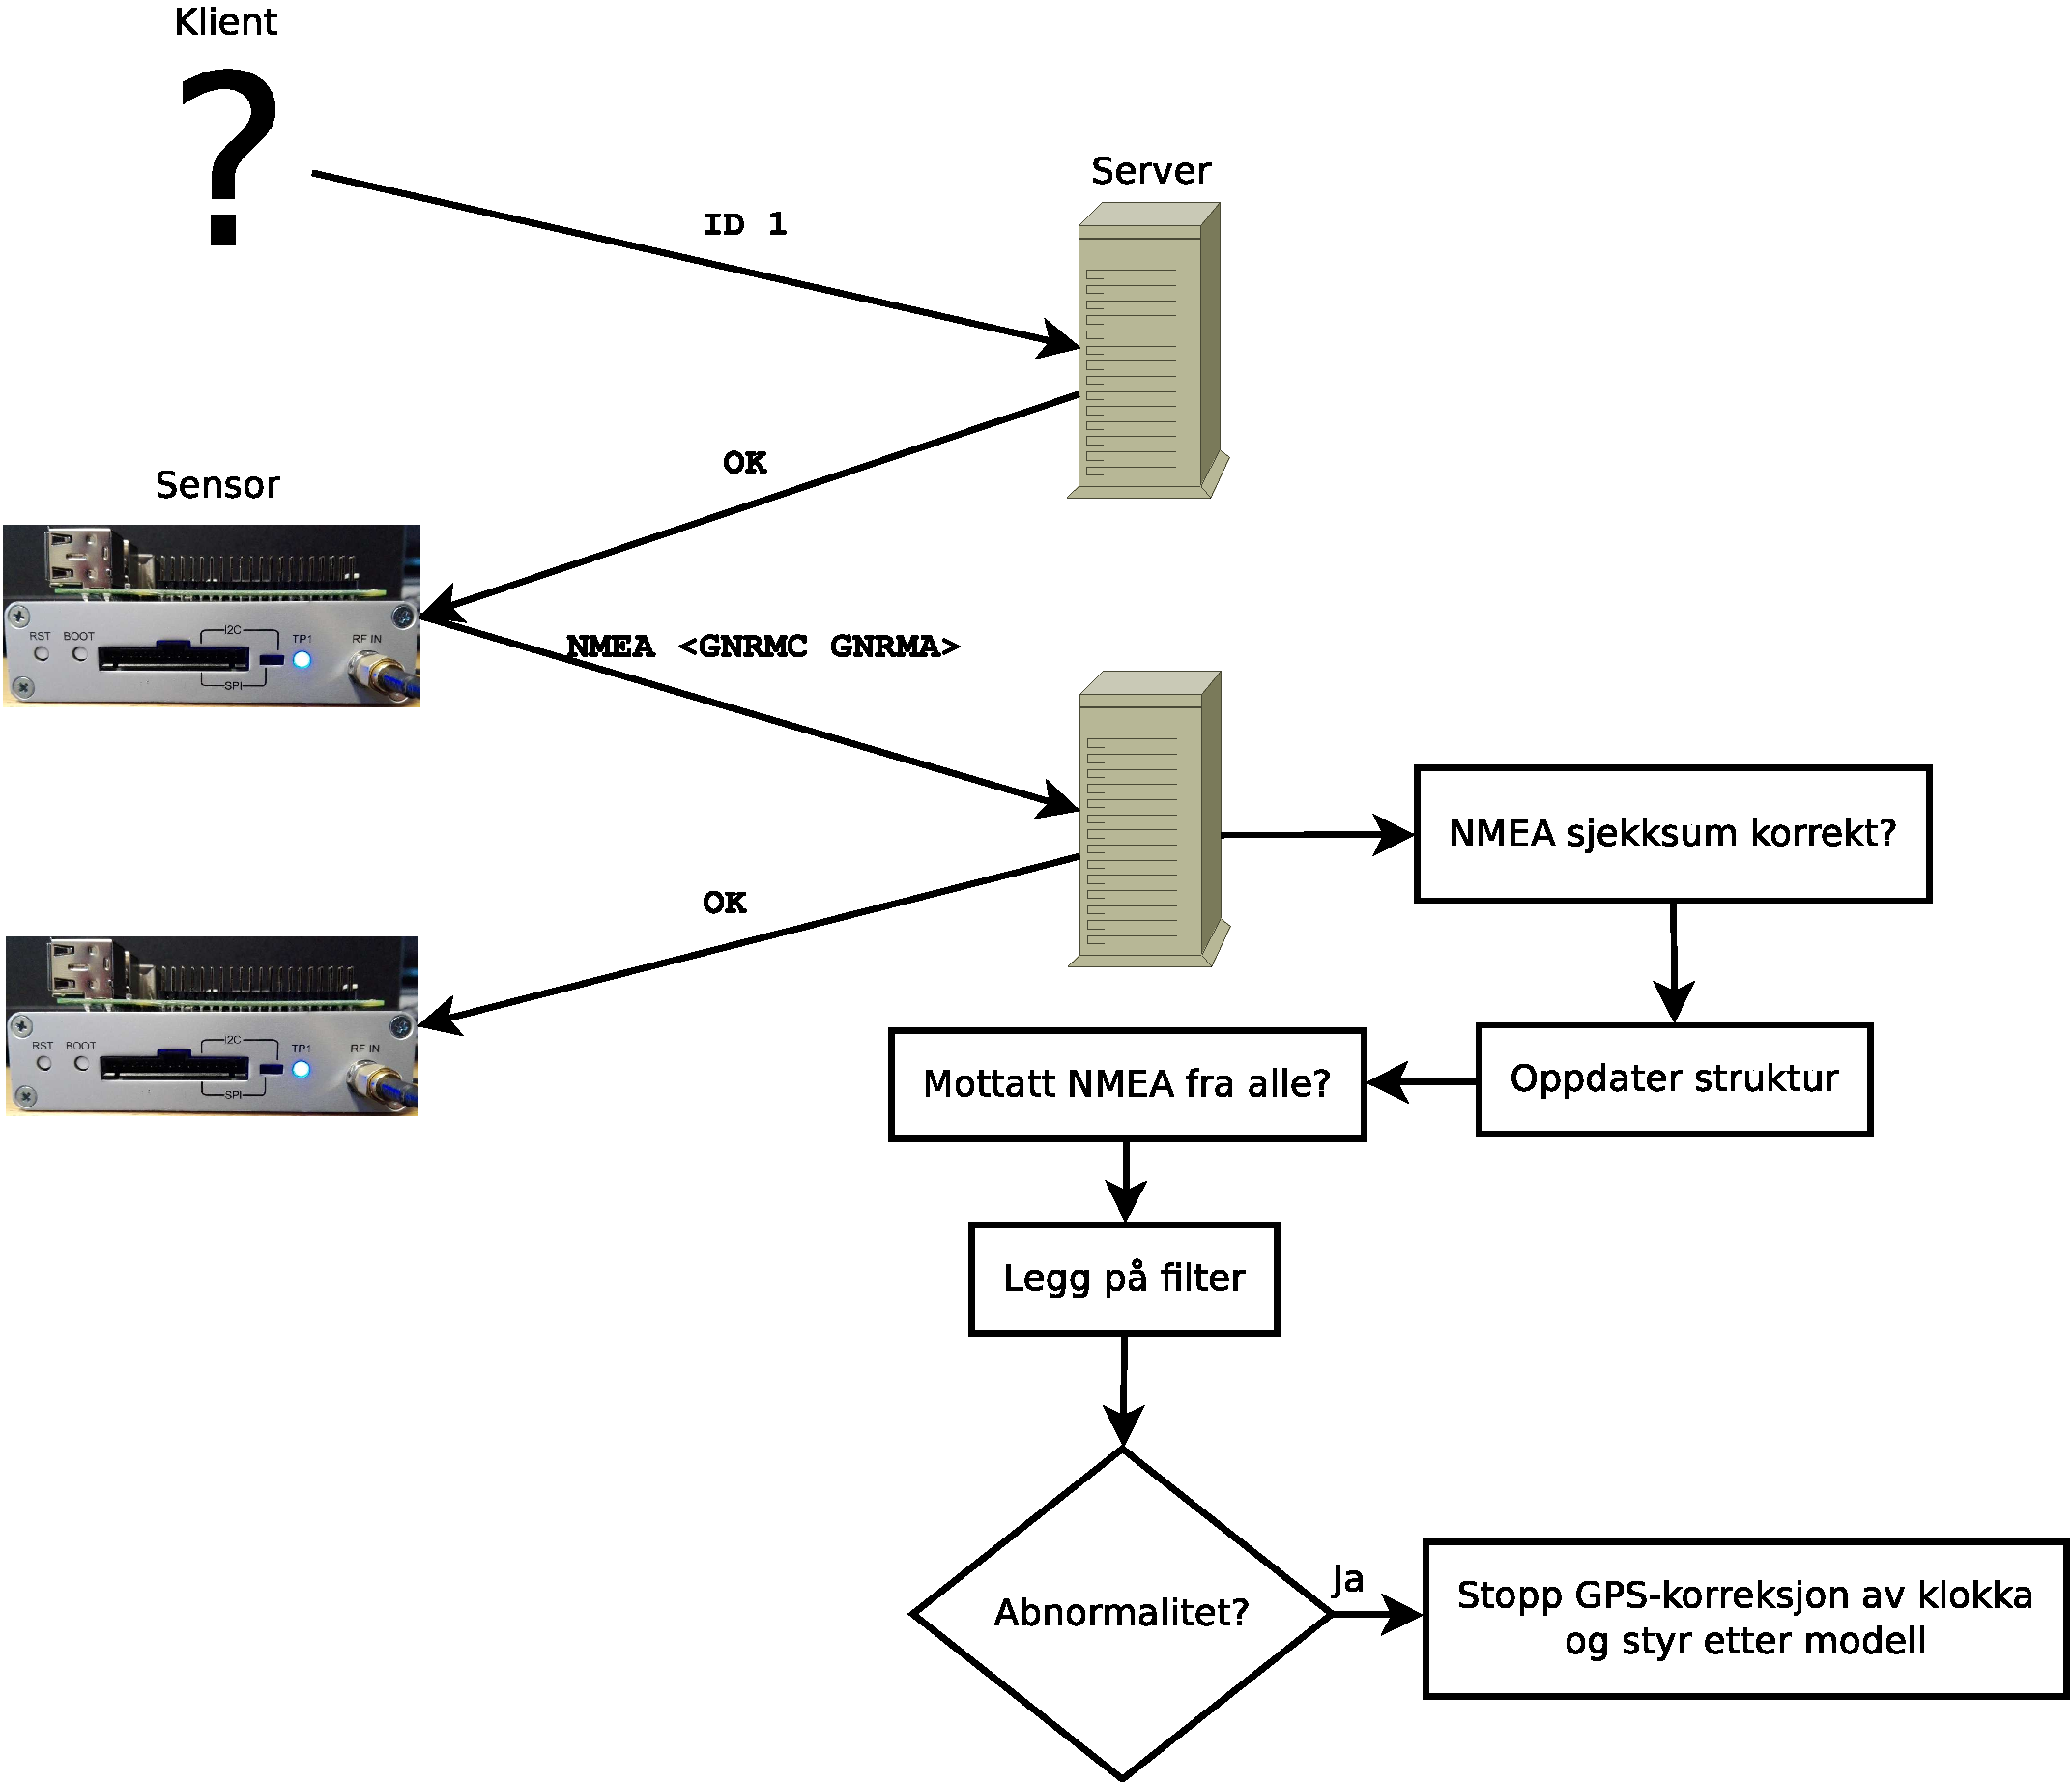
\includegraphics[scale=0.25]{thesis/graphics/sensor_nmea.pdf}
    \end{figure}
\end{frame}

\begin{frame}
\frametitle{Systemimplementasjon}
  \framesubtitle{Kommunikasjon: Bruker/Script}
    \begin{figure}
      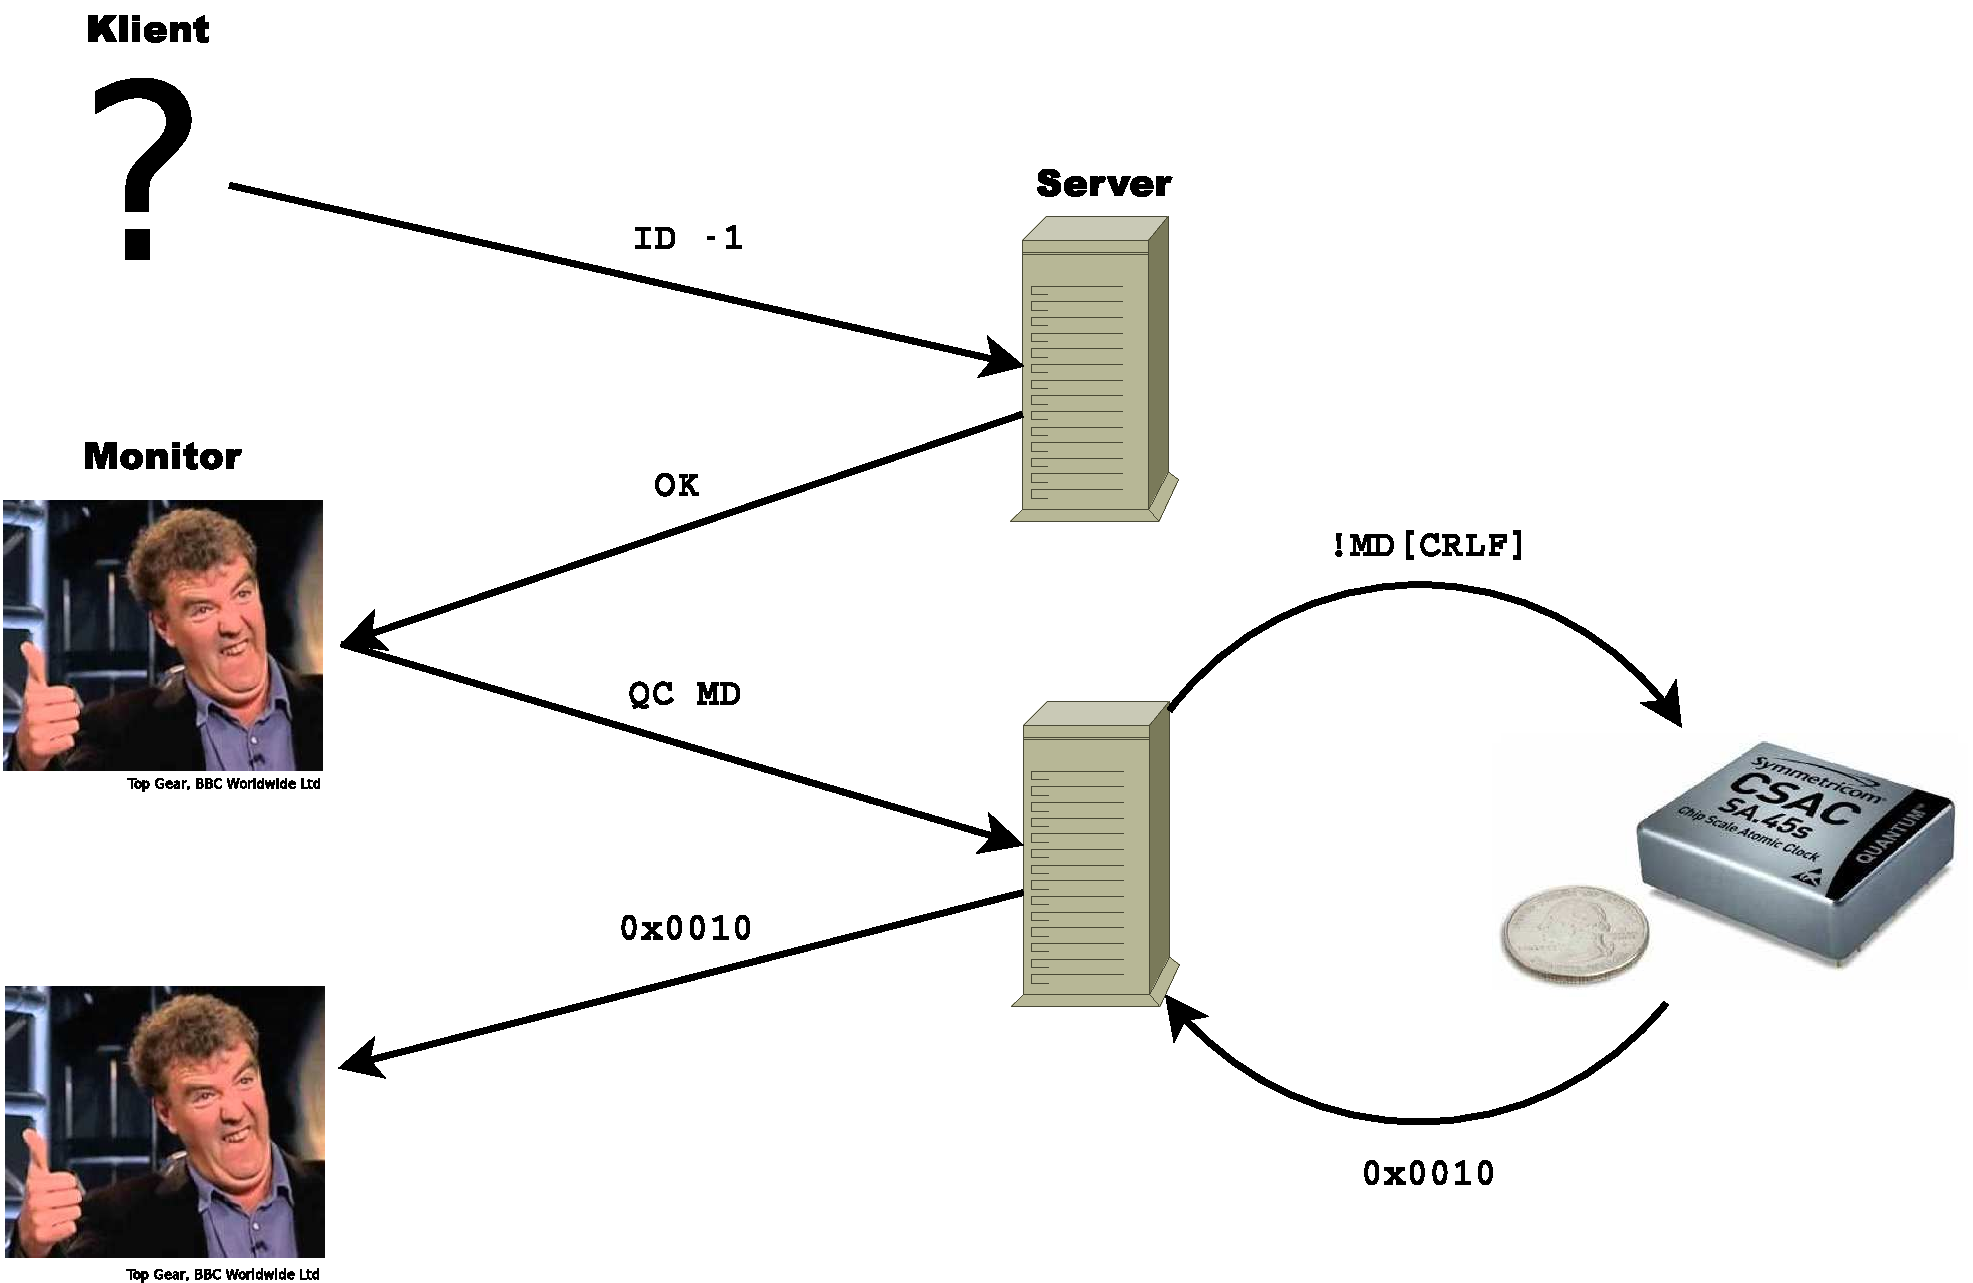
\includegraphics[scale=0.3]{thesis/graphics/monitor_csac_request.pdf}
    \end{figure}
\end{frame}

\section{Test av lokasjon- og hastighetsfilter}
\begin{frame}
\frametitle{Test av lokasjon- og hastighetsfilter}
\framesubtitle{Testoppsett: Konfigurasjon}
  \subsection{Beskrivelse}
      \begin{figure}
        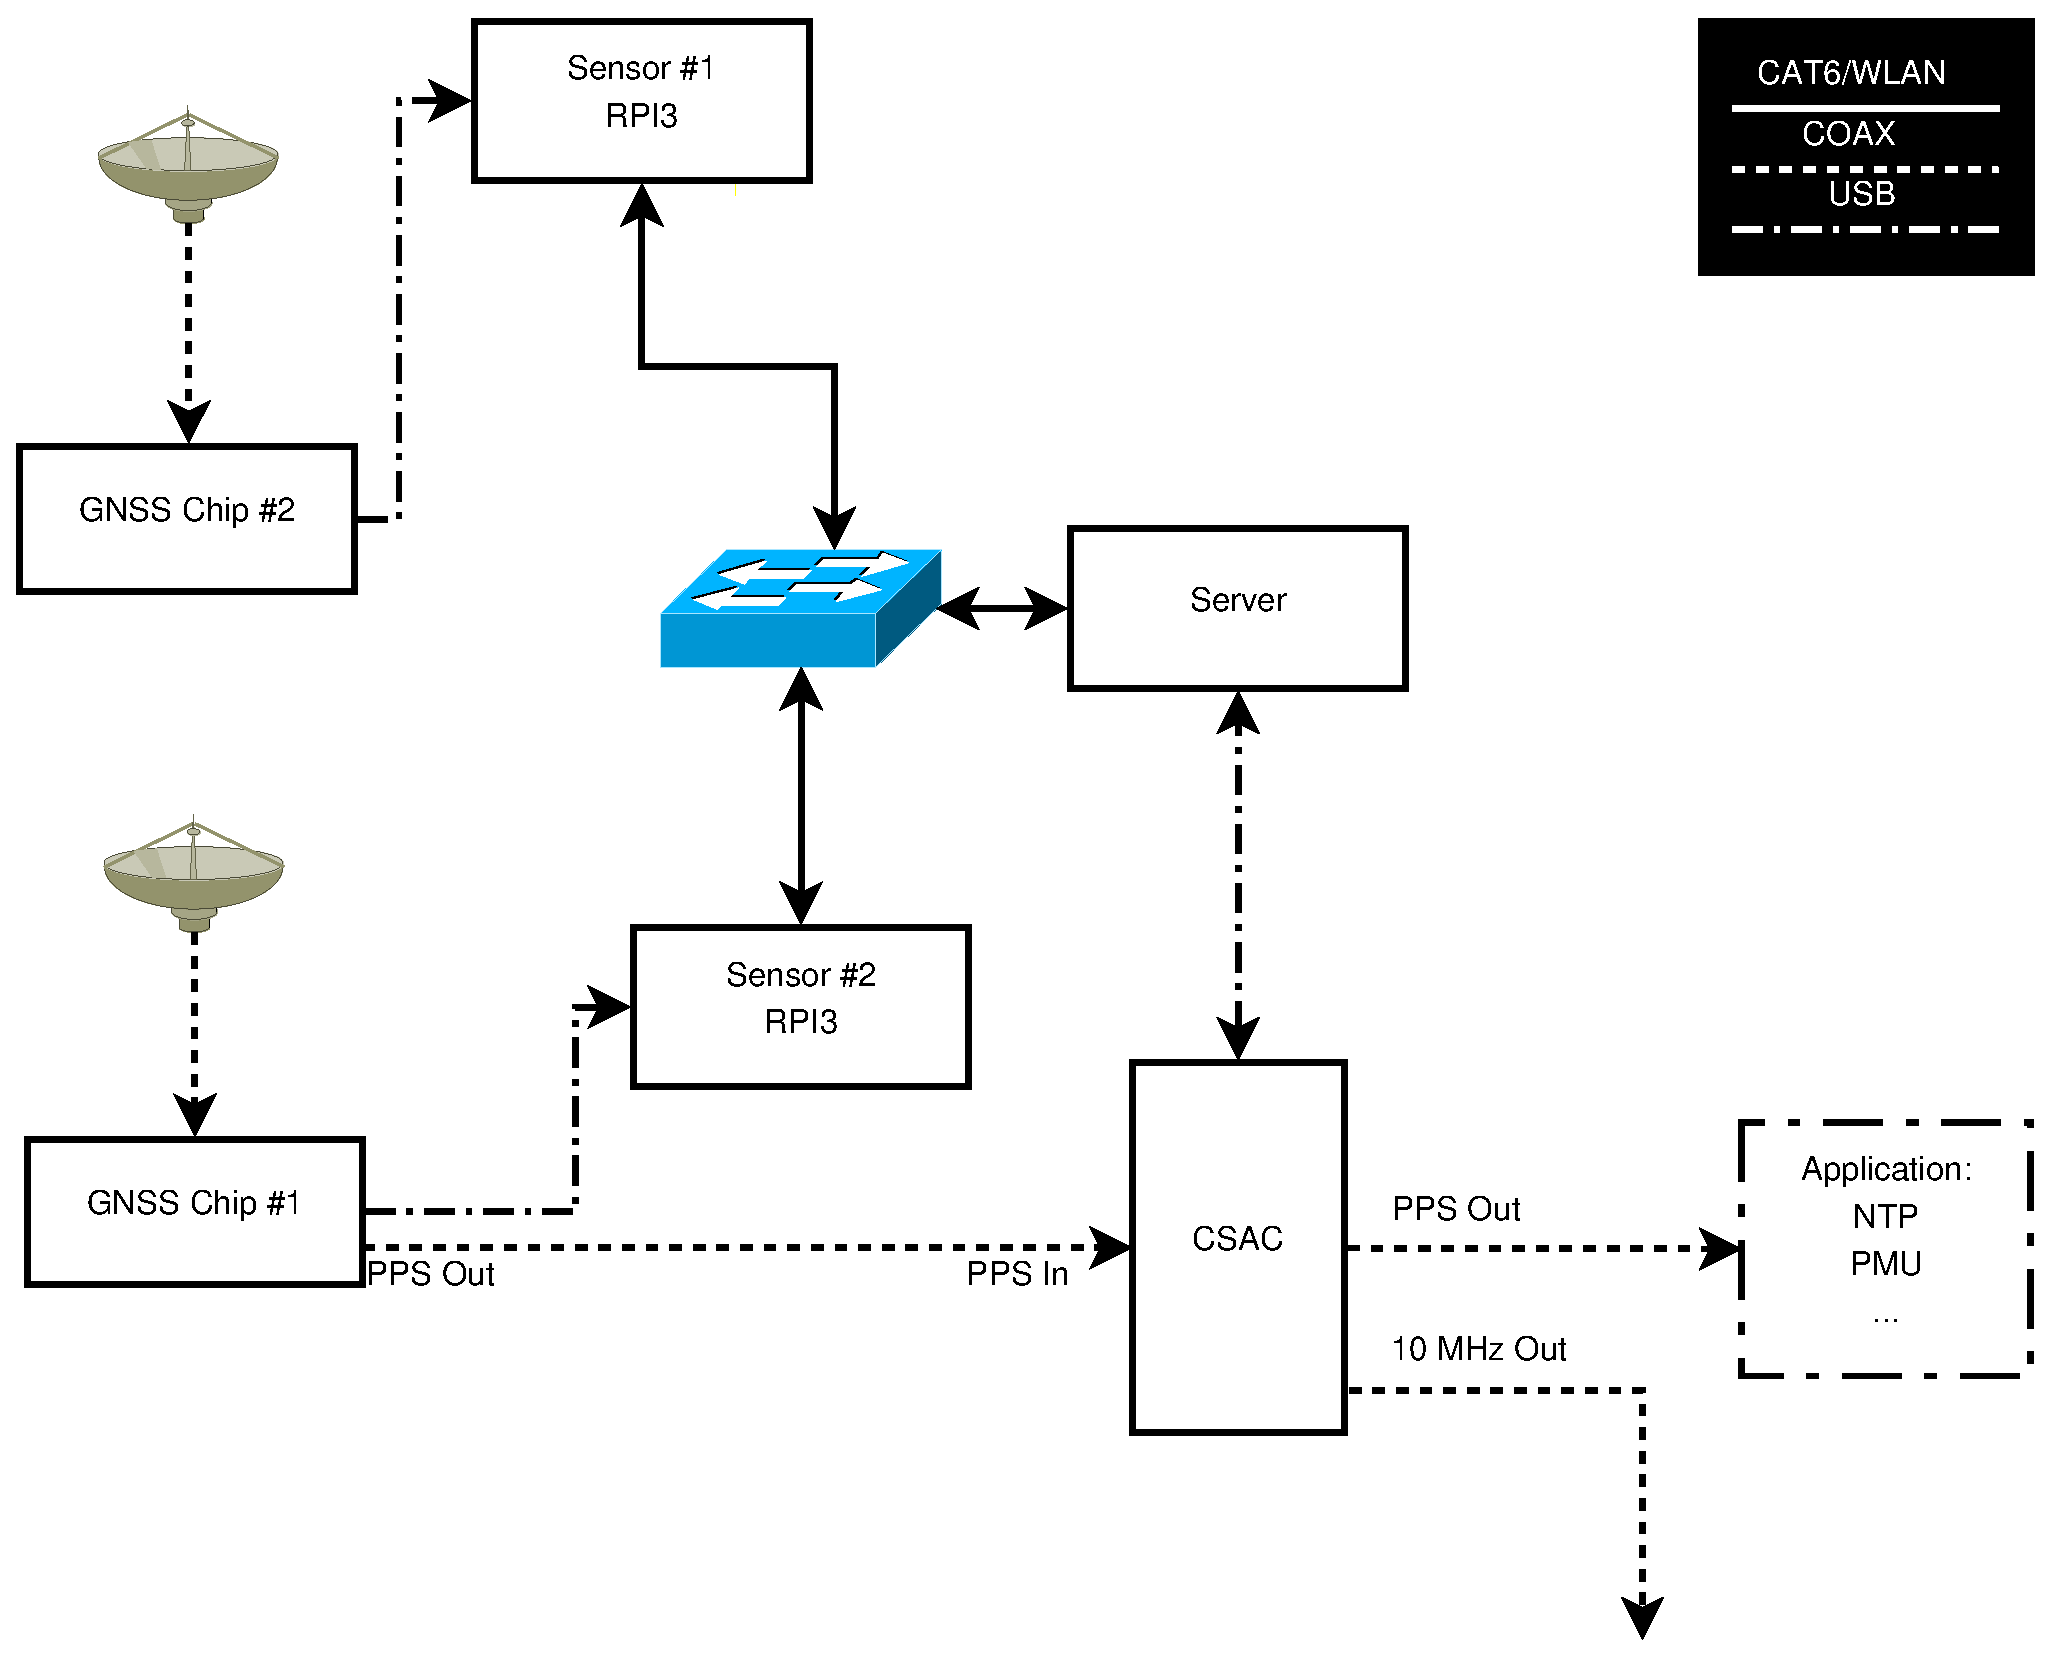
\includegraphics[scale=0.25]{thesis/graphics/server_layout.eps}
        \caption{Oppsett av server og klienter under test}
      \end{figure}
\end{frame}

\begin{frame}
\frametitle{Test av lokasjon- og hastighetsfilter}
\framesubtitle{Testoppsett: Måling}
      \begin{figure}
        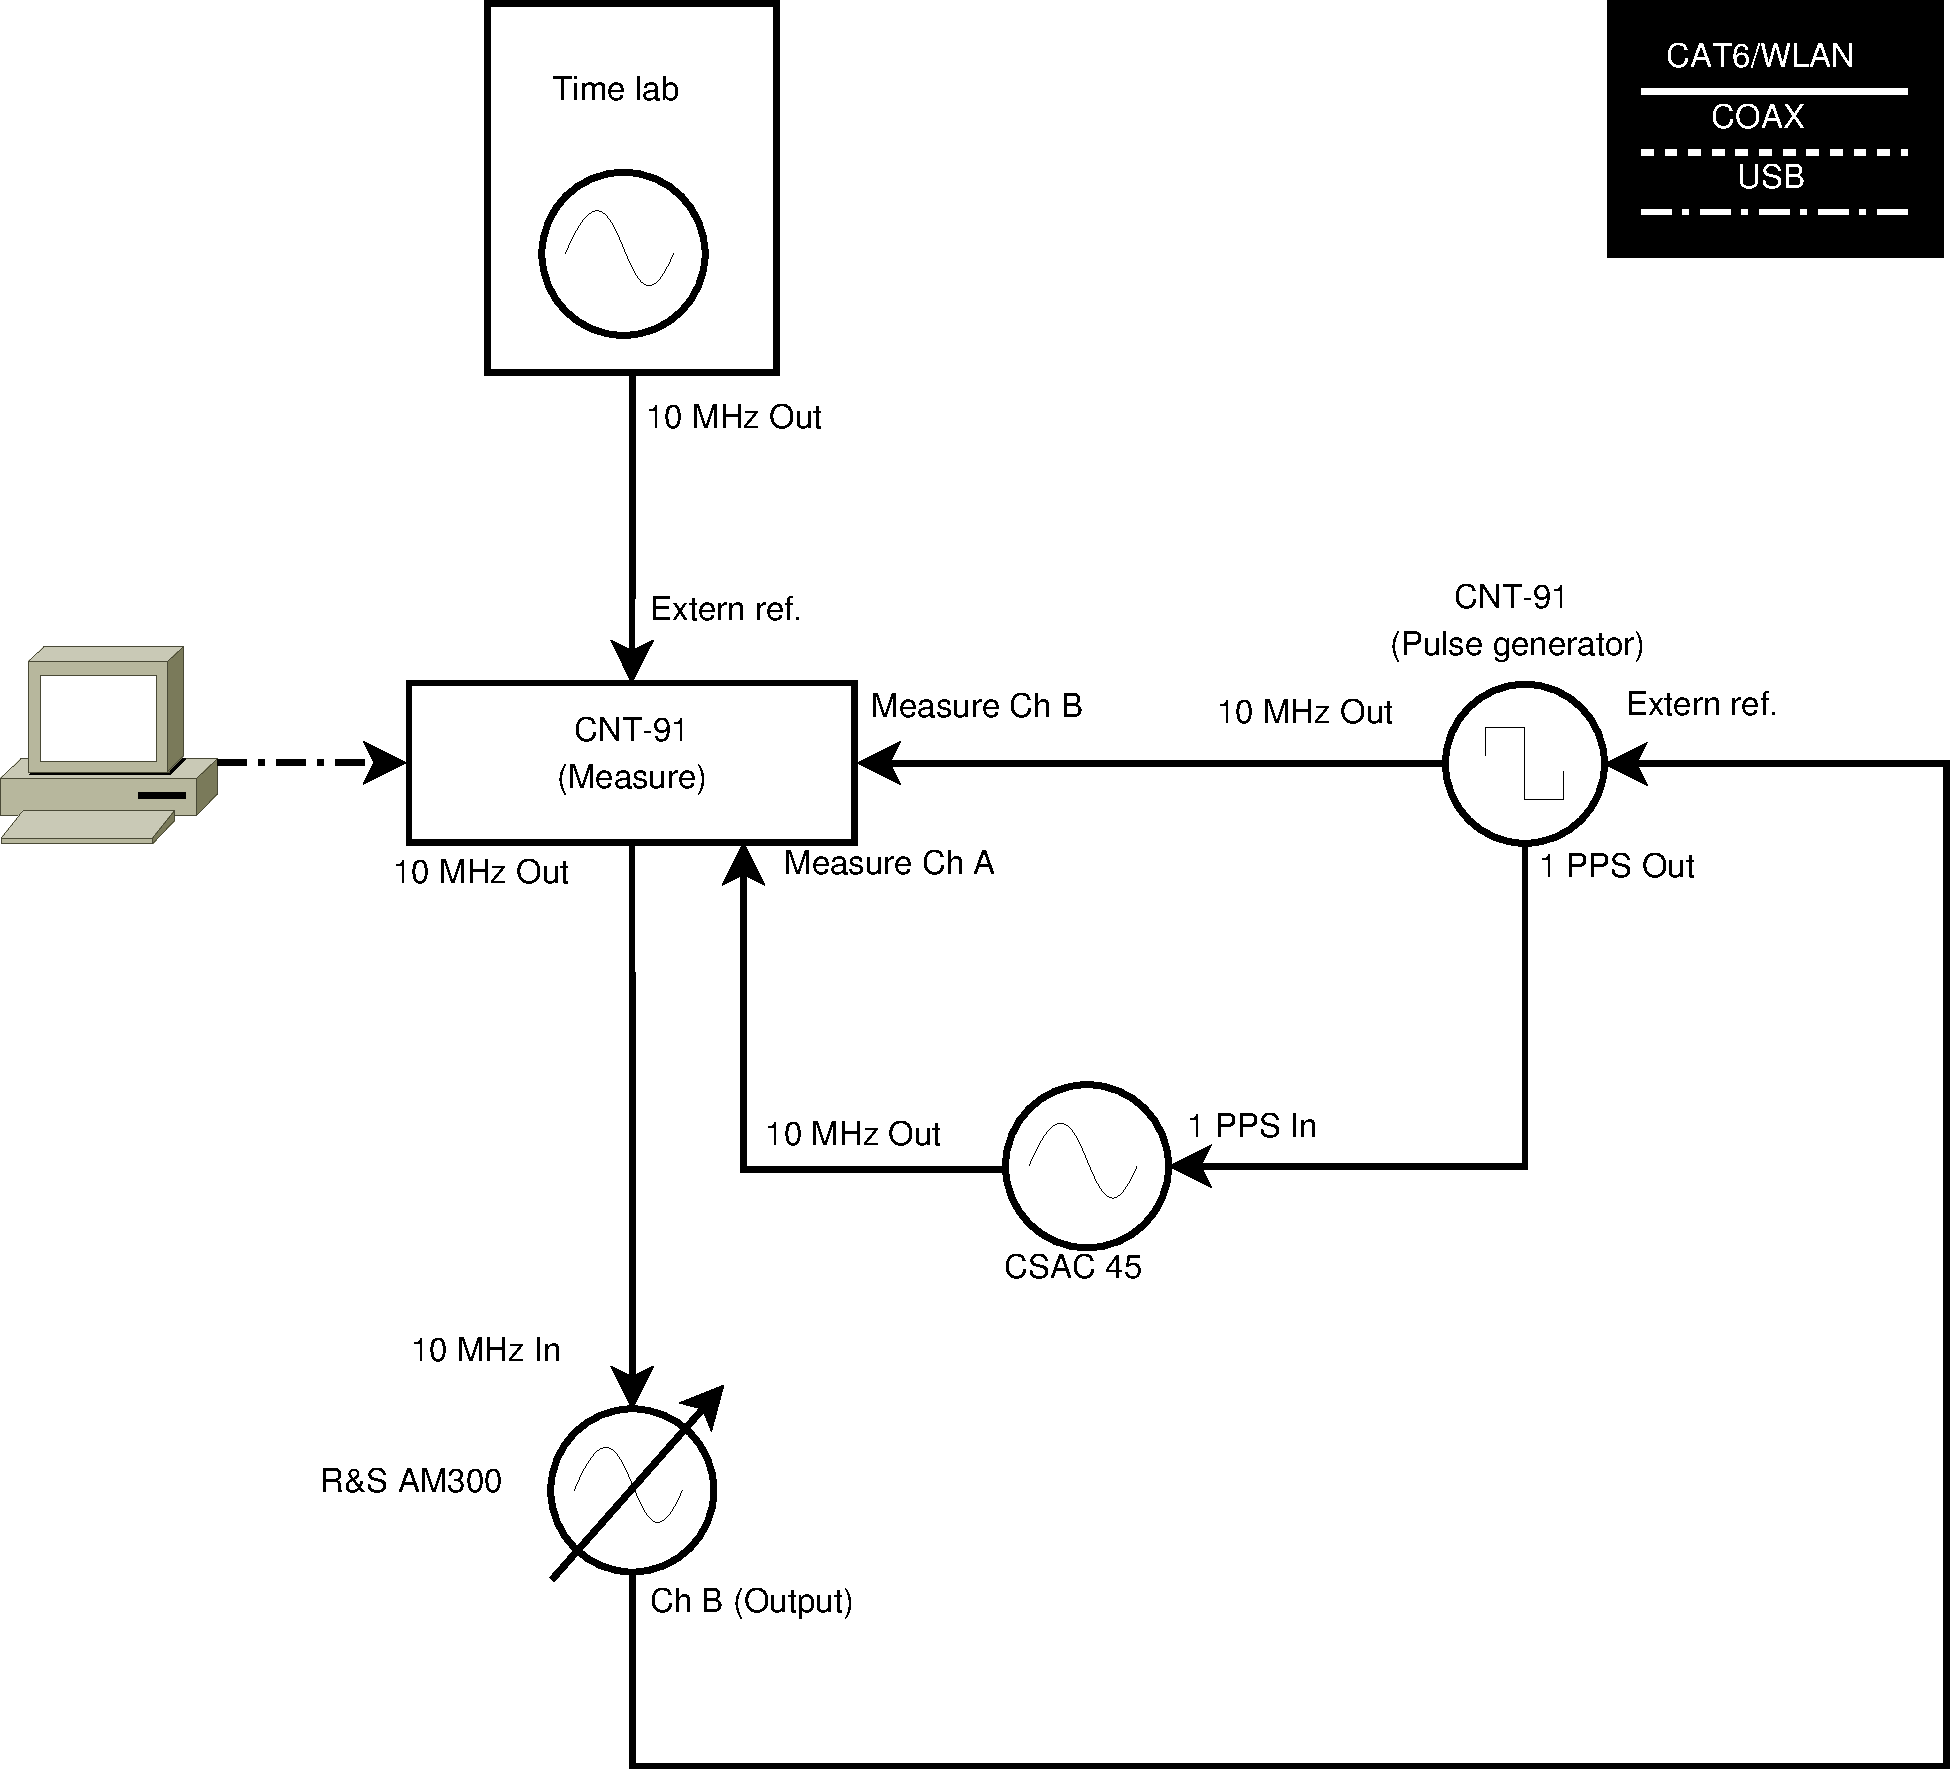
\includegraphics[scale=0.25]{thesis/graphics/measure_setup.pdf}
        \caption{Oppsett av måleutstyr}
      \end{figure}
\end{frame}

\begin{frame}
\frametitle{Test av lokasjon- og hastighetsfilter}
\framesubtitle{Testoppsett: Måling}
      \begin{figure}
        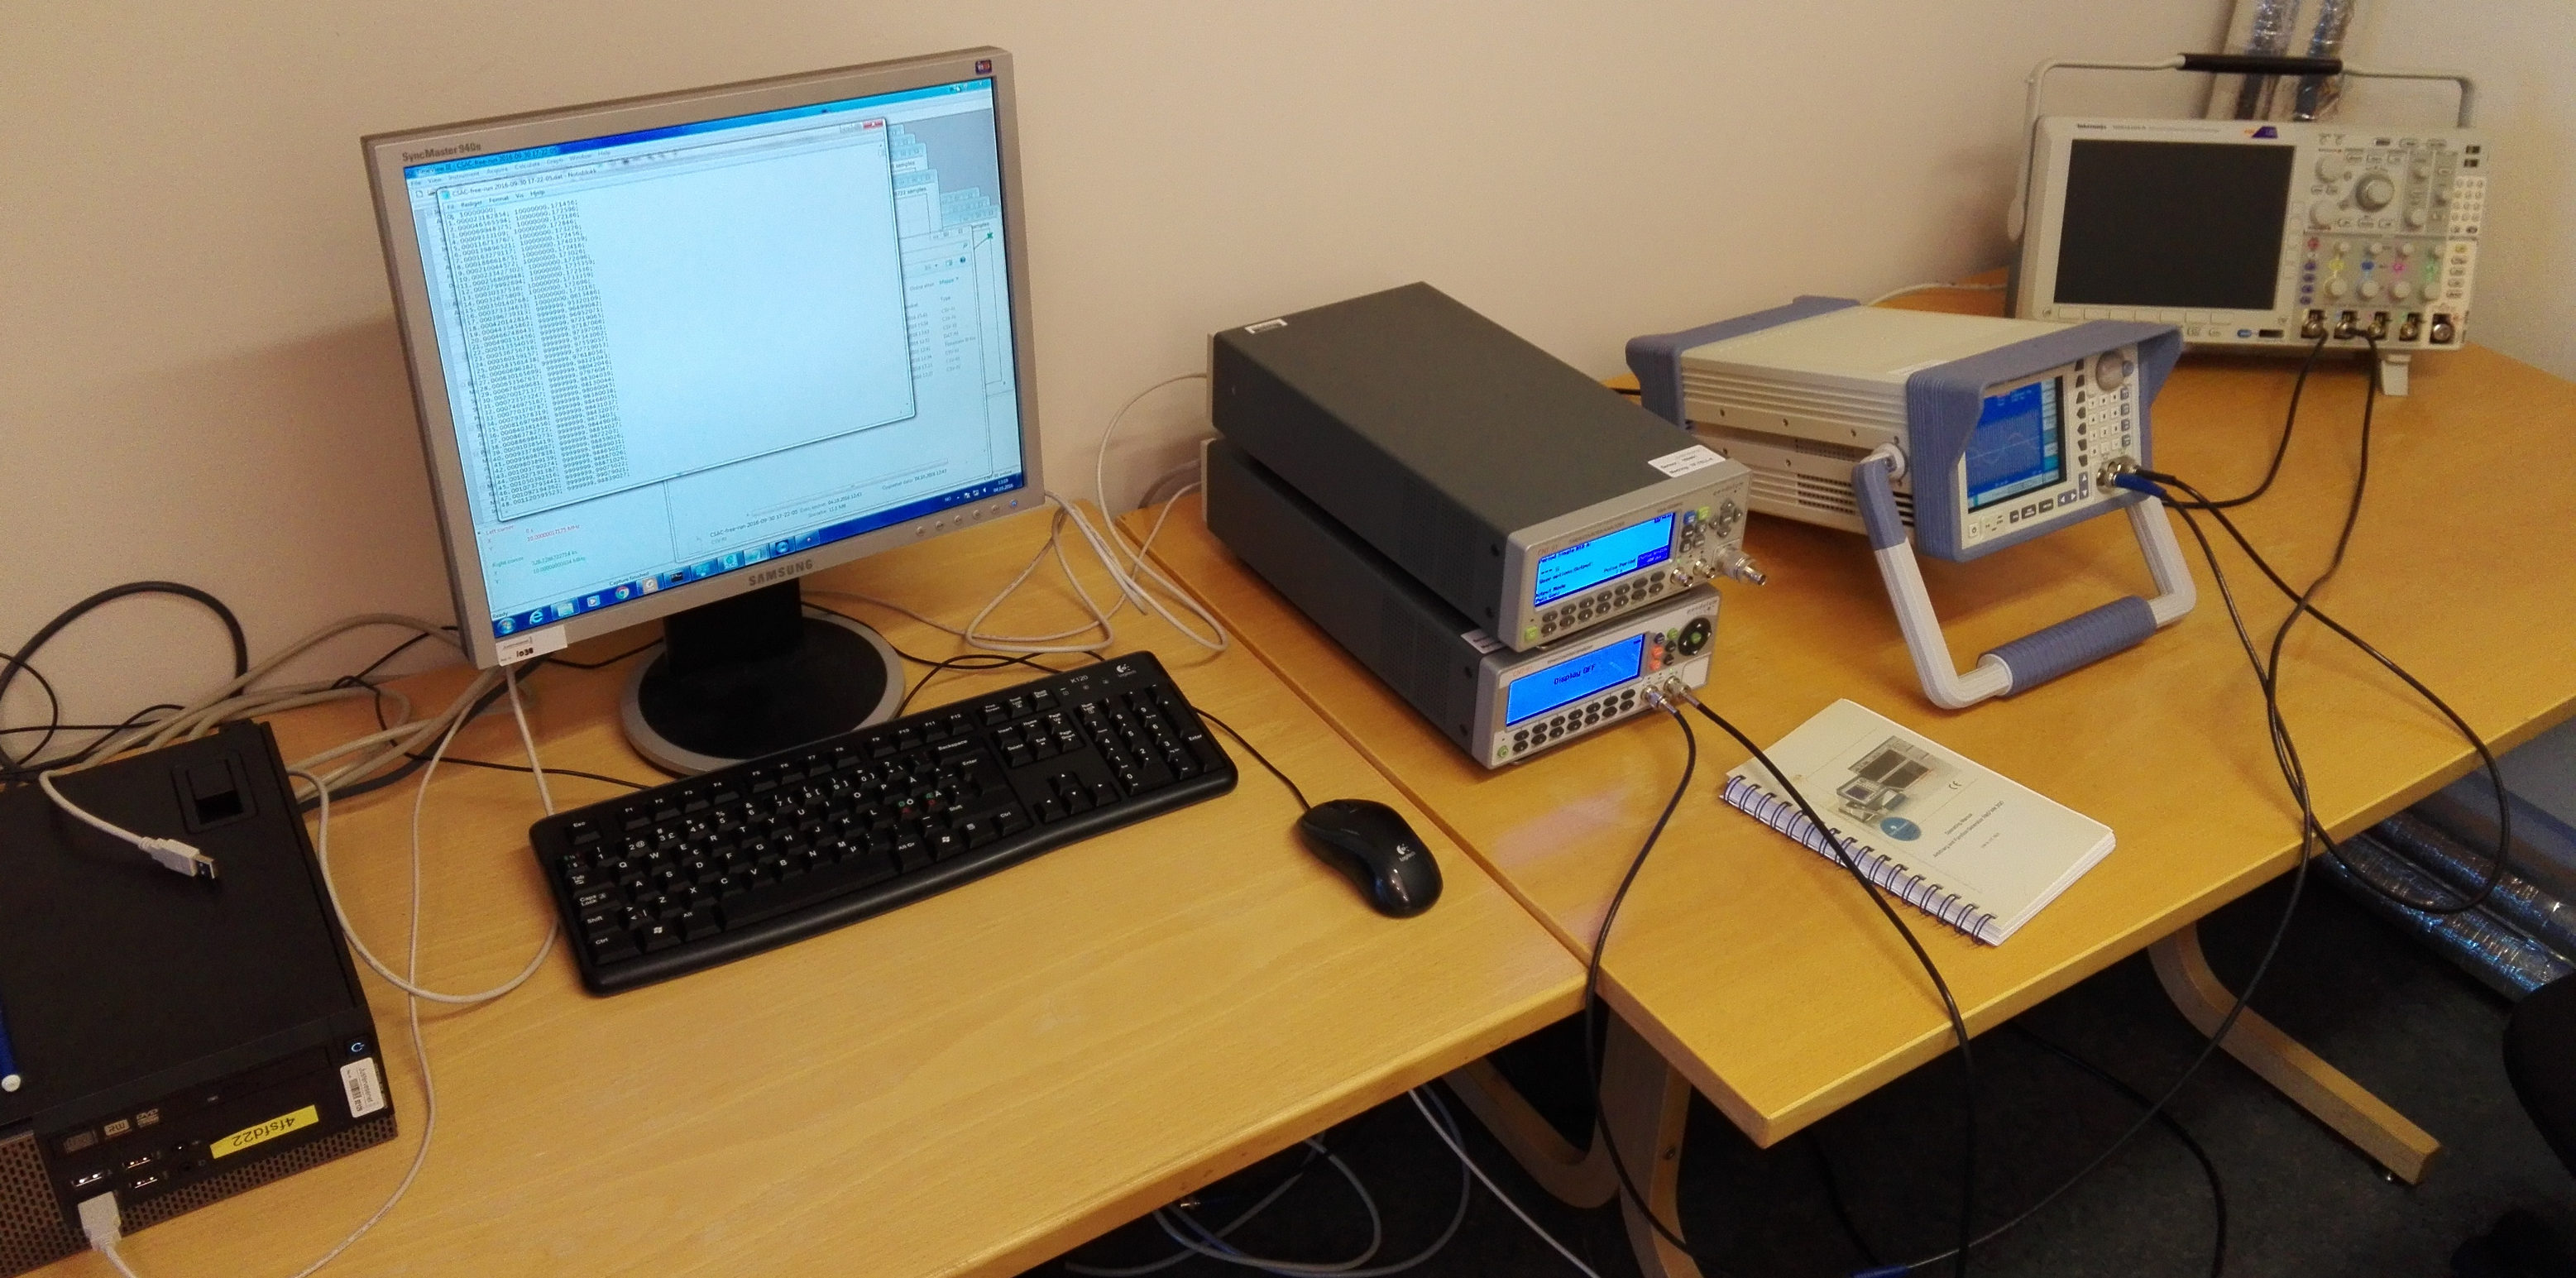
\includegraphics[scale=0.08]{thesis/graphics/lab_setup_cropped.jpg}
        \caption{Oppsett av måleutstyr}
      \end{figure}
\end{frame}

\begin{frame}
\frametitle{Test av lokasjon- og hastighetsfilter}
\framesubtitle{Testoppsett: Plassering av mottakere}
      \begin{figure}
        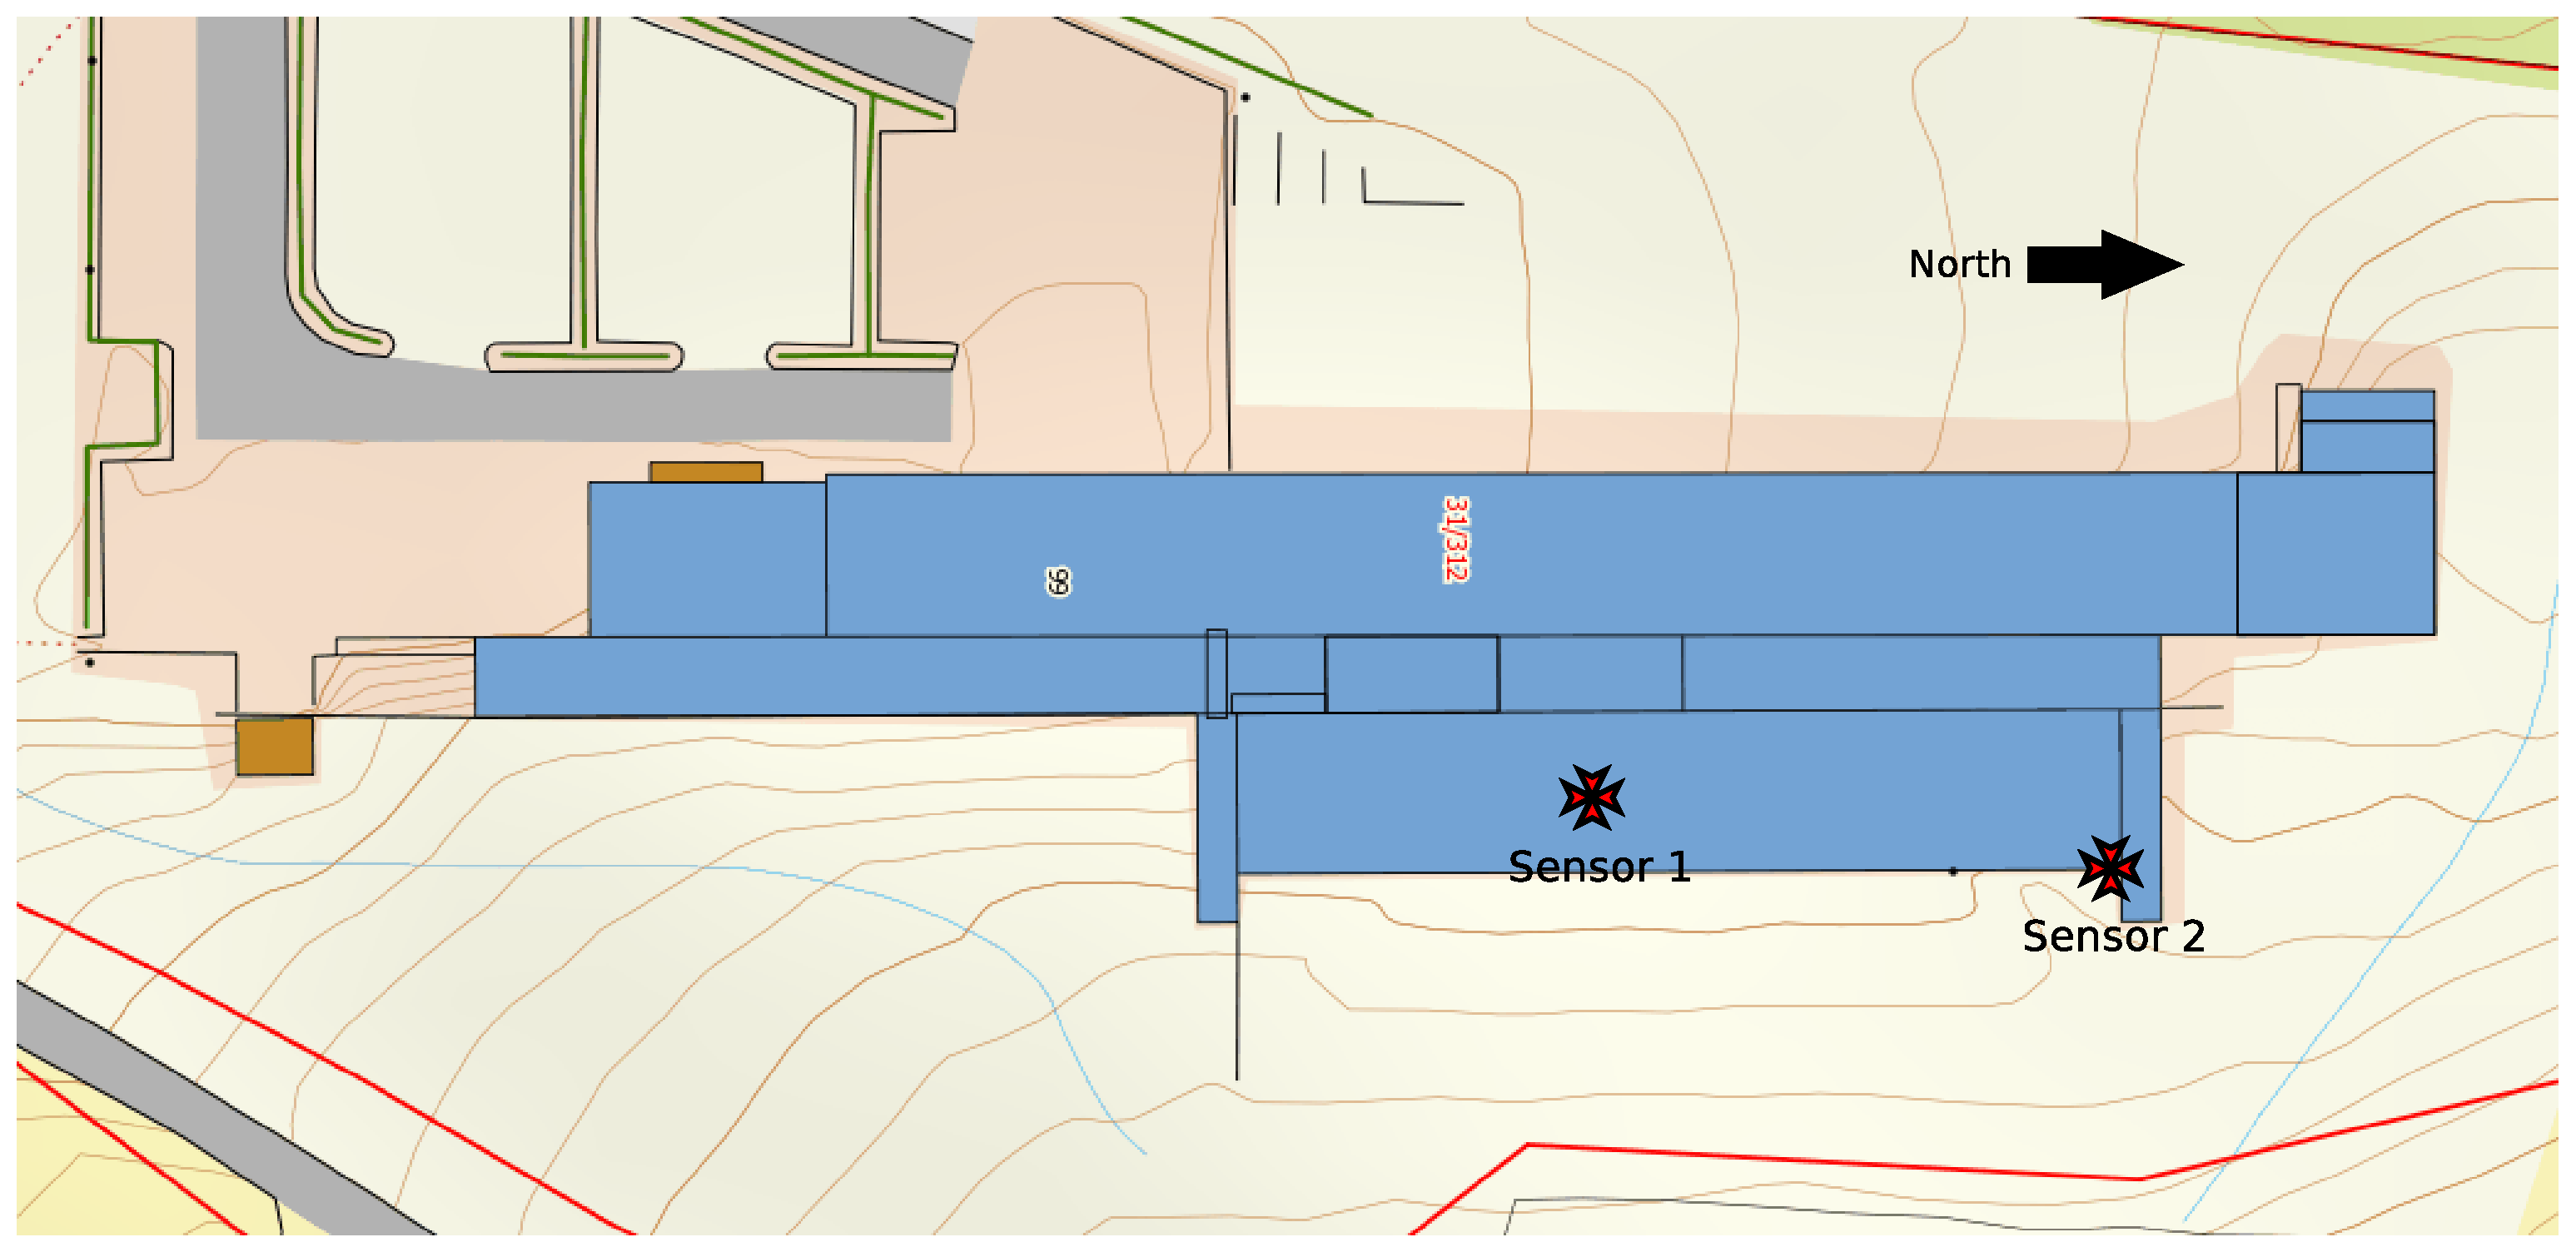
\includegraphics[scale=0.18]{thesis/graphics/roof.eps}
        \caption{Plasseringen av GPS-mottakere}
      \end{figure}
\end{frame}

\begin{frame}
\frametitle{Test av lokasjon- og hastighetsfilter}
\framesubtitle{Utførelse}
      \begin{itemize}
        \setlength\itemsep{2em}
        \item Flyttet antenne 1 mot antenne 2
        \item Flyttet antenne 2 mot antenne 1
        \item Viftet antenne 1 rundt i en halvsirkel
        \item Viftet antenne 2 rundt i en halvsirkel
        \item Dekket antennene
      \end{itemize}
\end{frame}

\begin{frame}
\frametitle{Test av lokasjon- og hastighetsfilter}
\framesubtitle{Utførelse}
\begin{center}
\begin{tikzpicture}
  \node (img1) {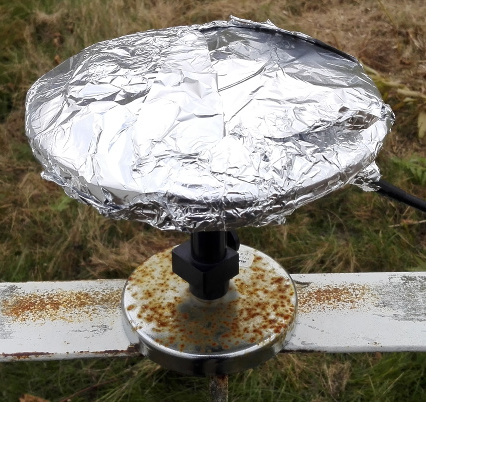
\includegraphics[height=5cm]{thesis/graphics/antenna_foil_over_hacked.jpg}};
  \node (img2) at (img1.south east) {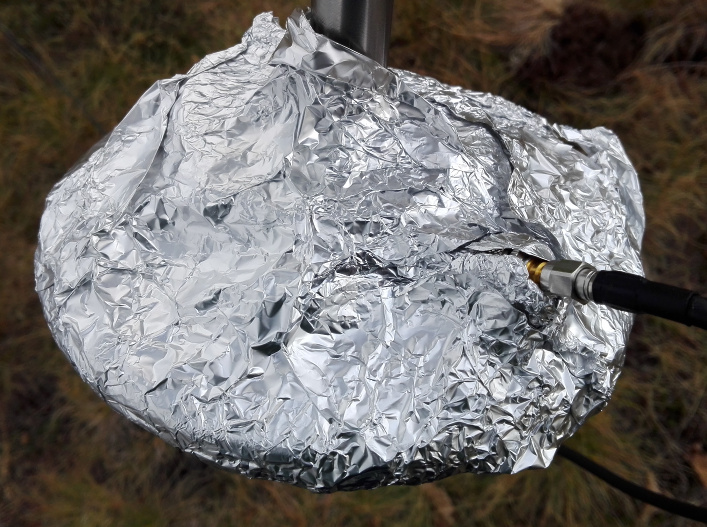
\includegraphics[height=4.5cm]{thesis/graphics/antenna_foil_cover.jpg}};
\end{tikzpicture}
\end{center}
\end{frame}

\begin{frame}
\frametitle{Test av lokasjon- og hastighetsfilter}
\framesubtitle{Observasjon}
      \begin{figure}
        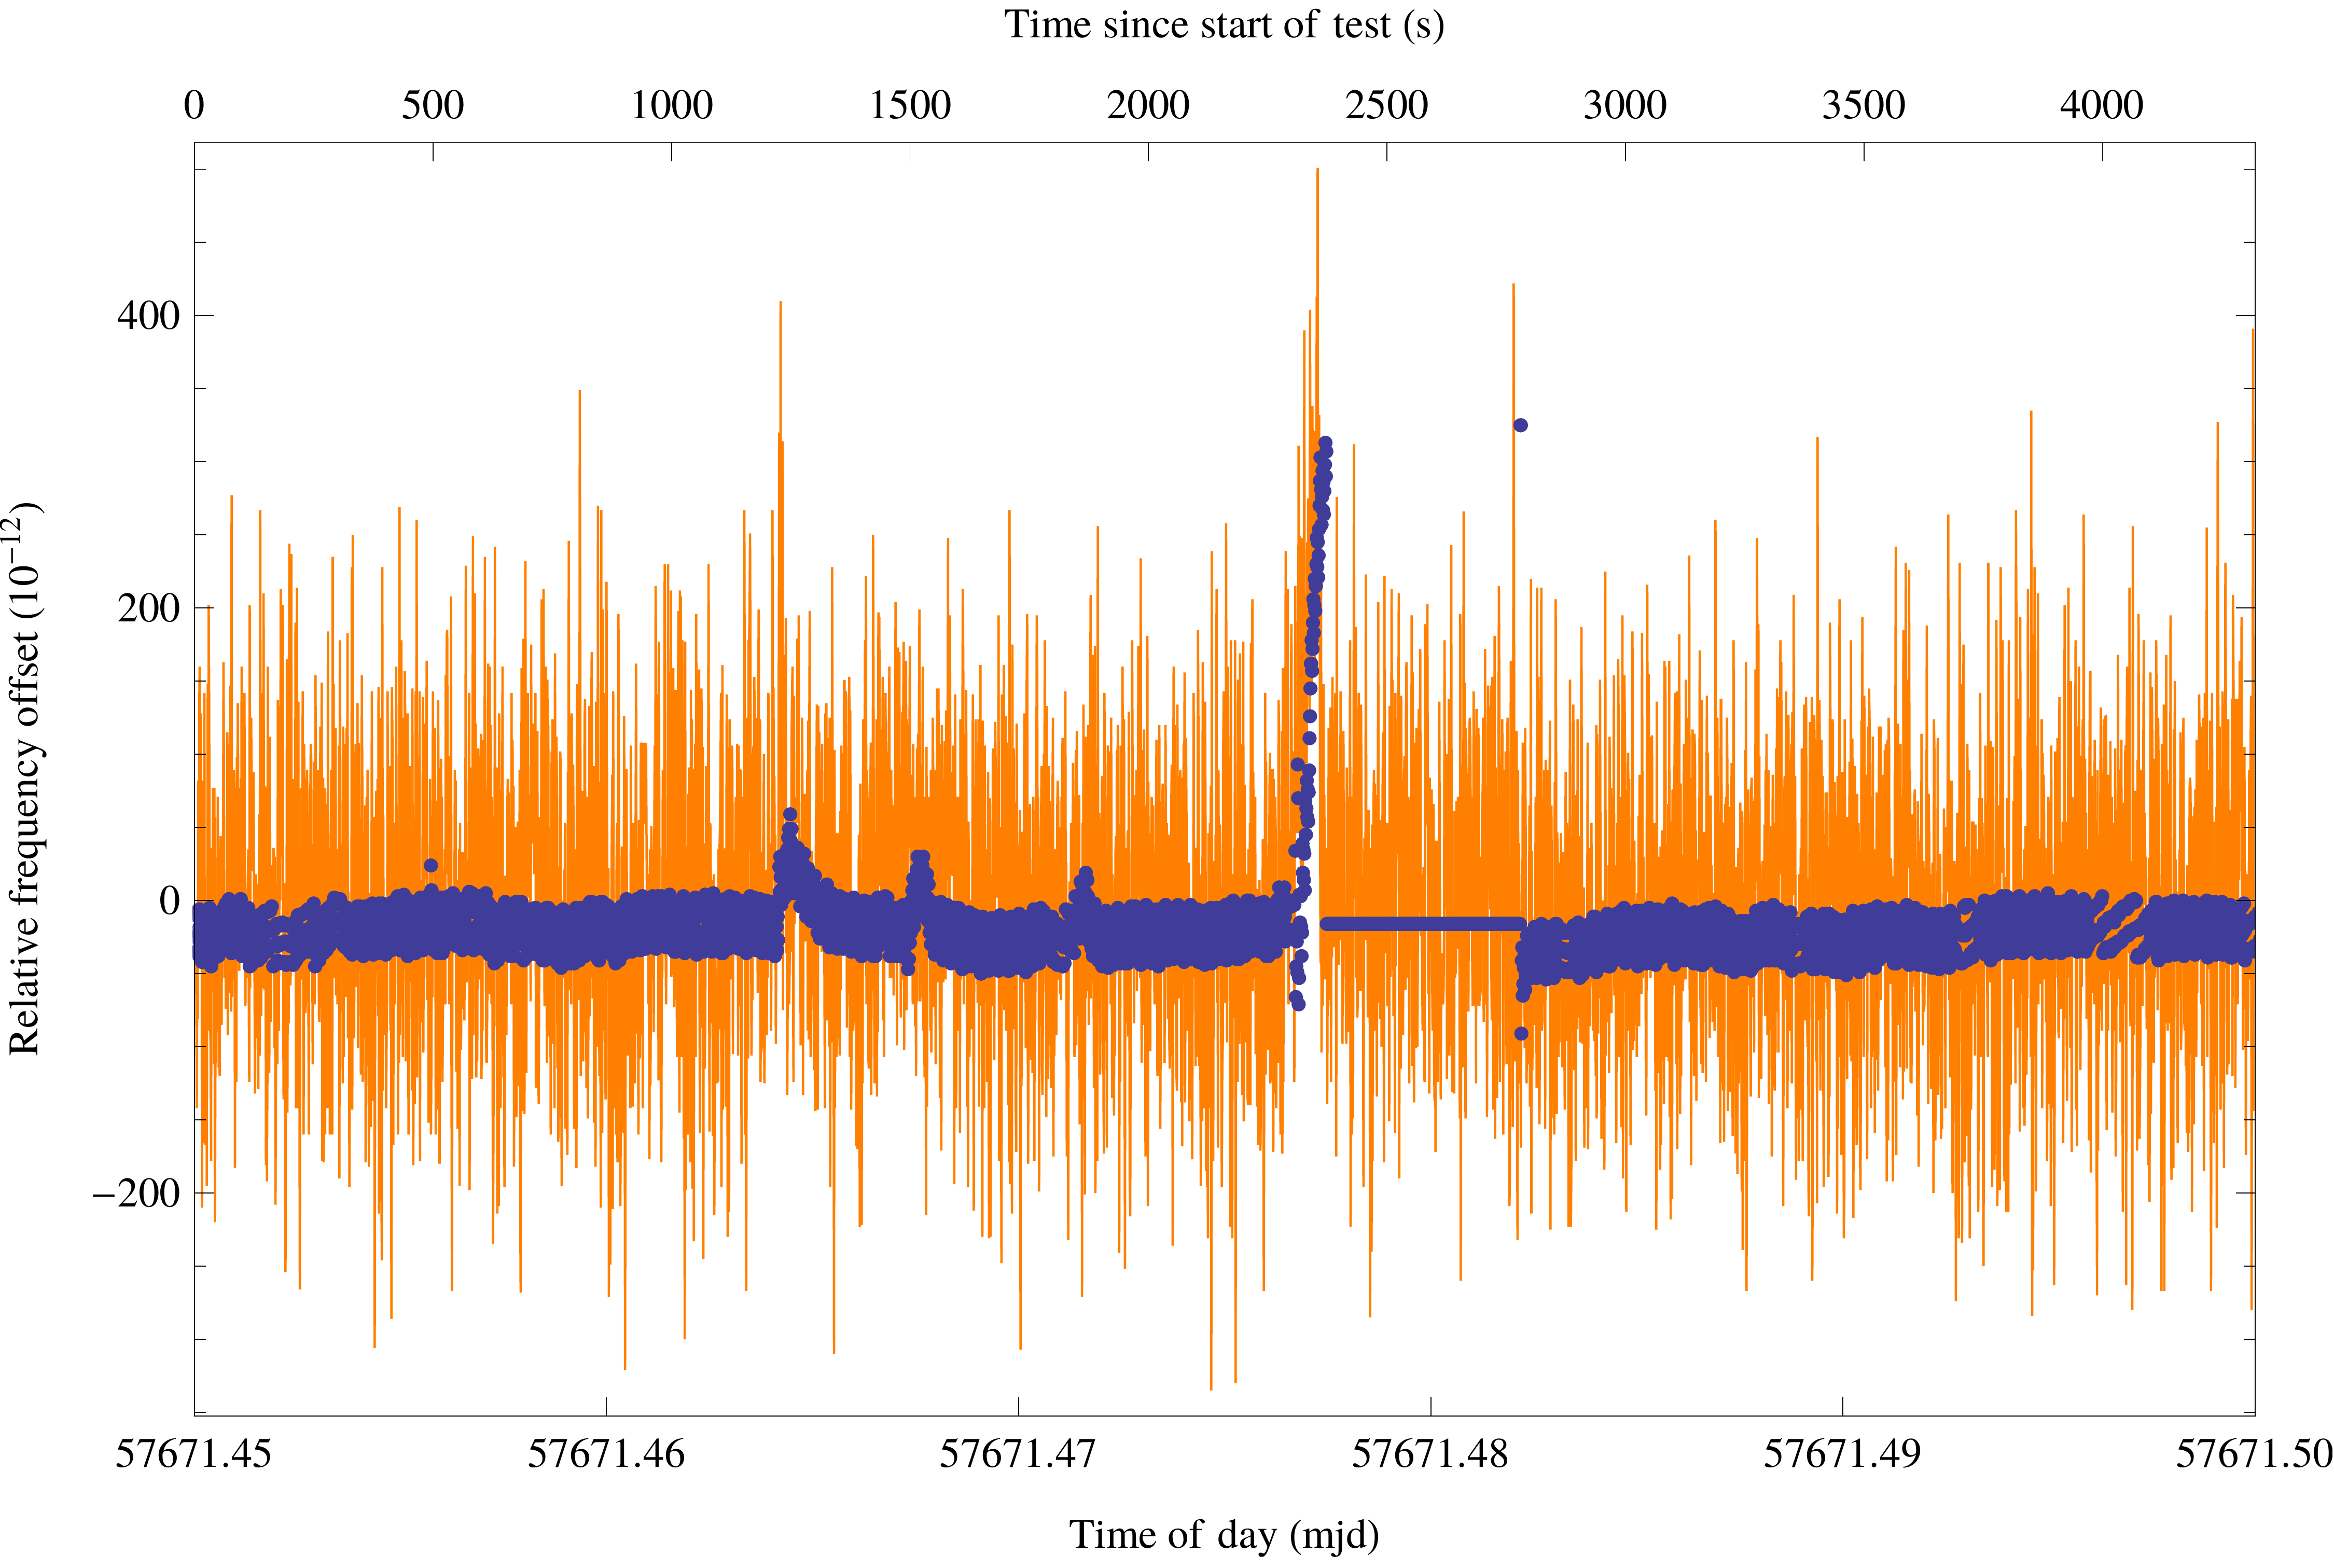
\includegraphics[scale=0.70]{thesis/graphics/cns91-and-csac-telemetry-frequency-1.png}
        \caption{Måleserie gjort under test av lokasjon og hastighetsfilter}
      \end{figure}
\end{frame}

\section{Test av klokkemodell og filtre}
\begin{frame}
\frametitle{Test av klokkemodell og filtre}
\framesubtitle{Oppsett}
  \begin{itemize}
        \setlength\itemsep{2em}
    \item Testet klokkemodellen og styring.
    \item Tok bare med en Sensor da fokus var på klokkemodell. 
  \end{itemize}
\end{frame}

\begin{frame}
\frametitle{Test av klokkemodell og filtre}
\framesubtitle{Utførelse}
      \begin{itemize}
            \setlength\itemsep{2em}
        \item Flyttet antenne 
        \item Viftet antenne rundt i en halvsirkel
      \end{itemize}
\end{frame}

\begin{frame}
\frametitle{Test av klokkemodell og filtre}
\framesubtitle{Observasjon}
      \begin{figure}
        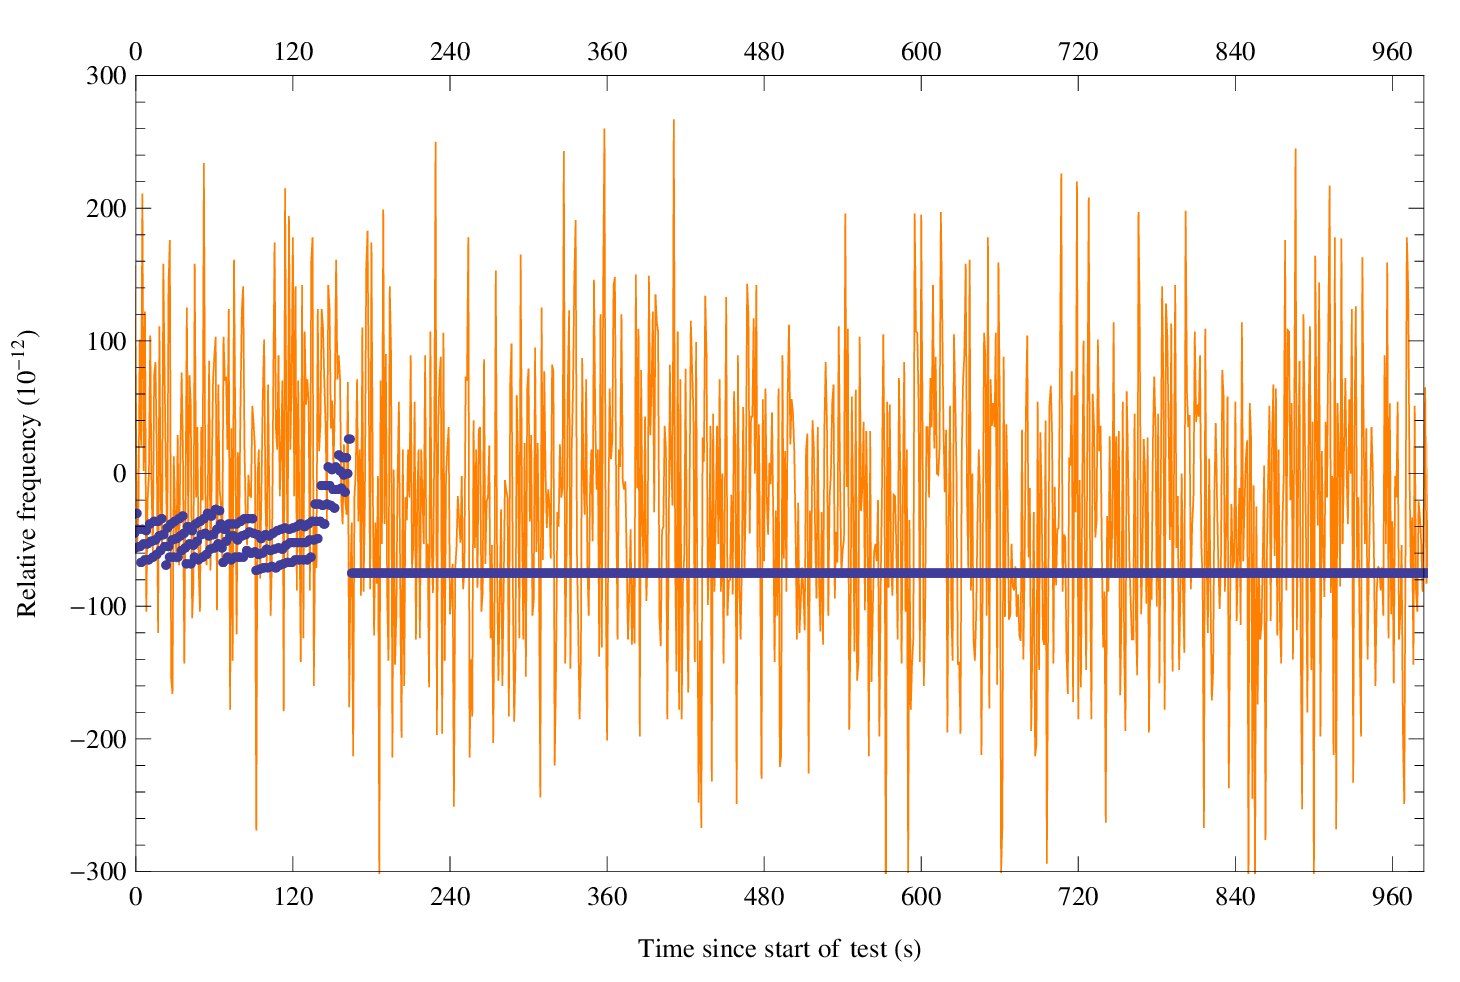
\includegraphics[scale=0.18]{thesis/graphics/20161024-test2-telemetry-and-cnt91-combined-1-3.png}
        \caption{Måleserie gjort under klokkemodell test}
      \end{figure}
\end{frame}

\begin{frame}
\section{Utilsiktet forstyrrelse}
\frametitle{Utilsiktet forstyrrelse}
      \begin{figure}
        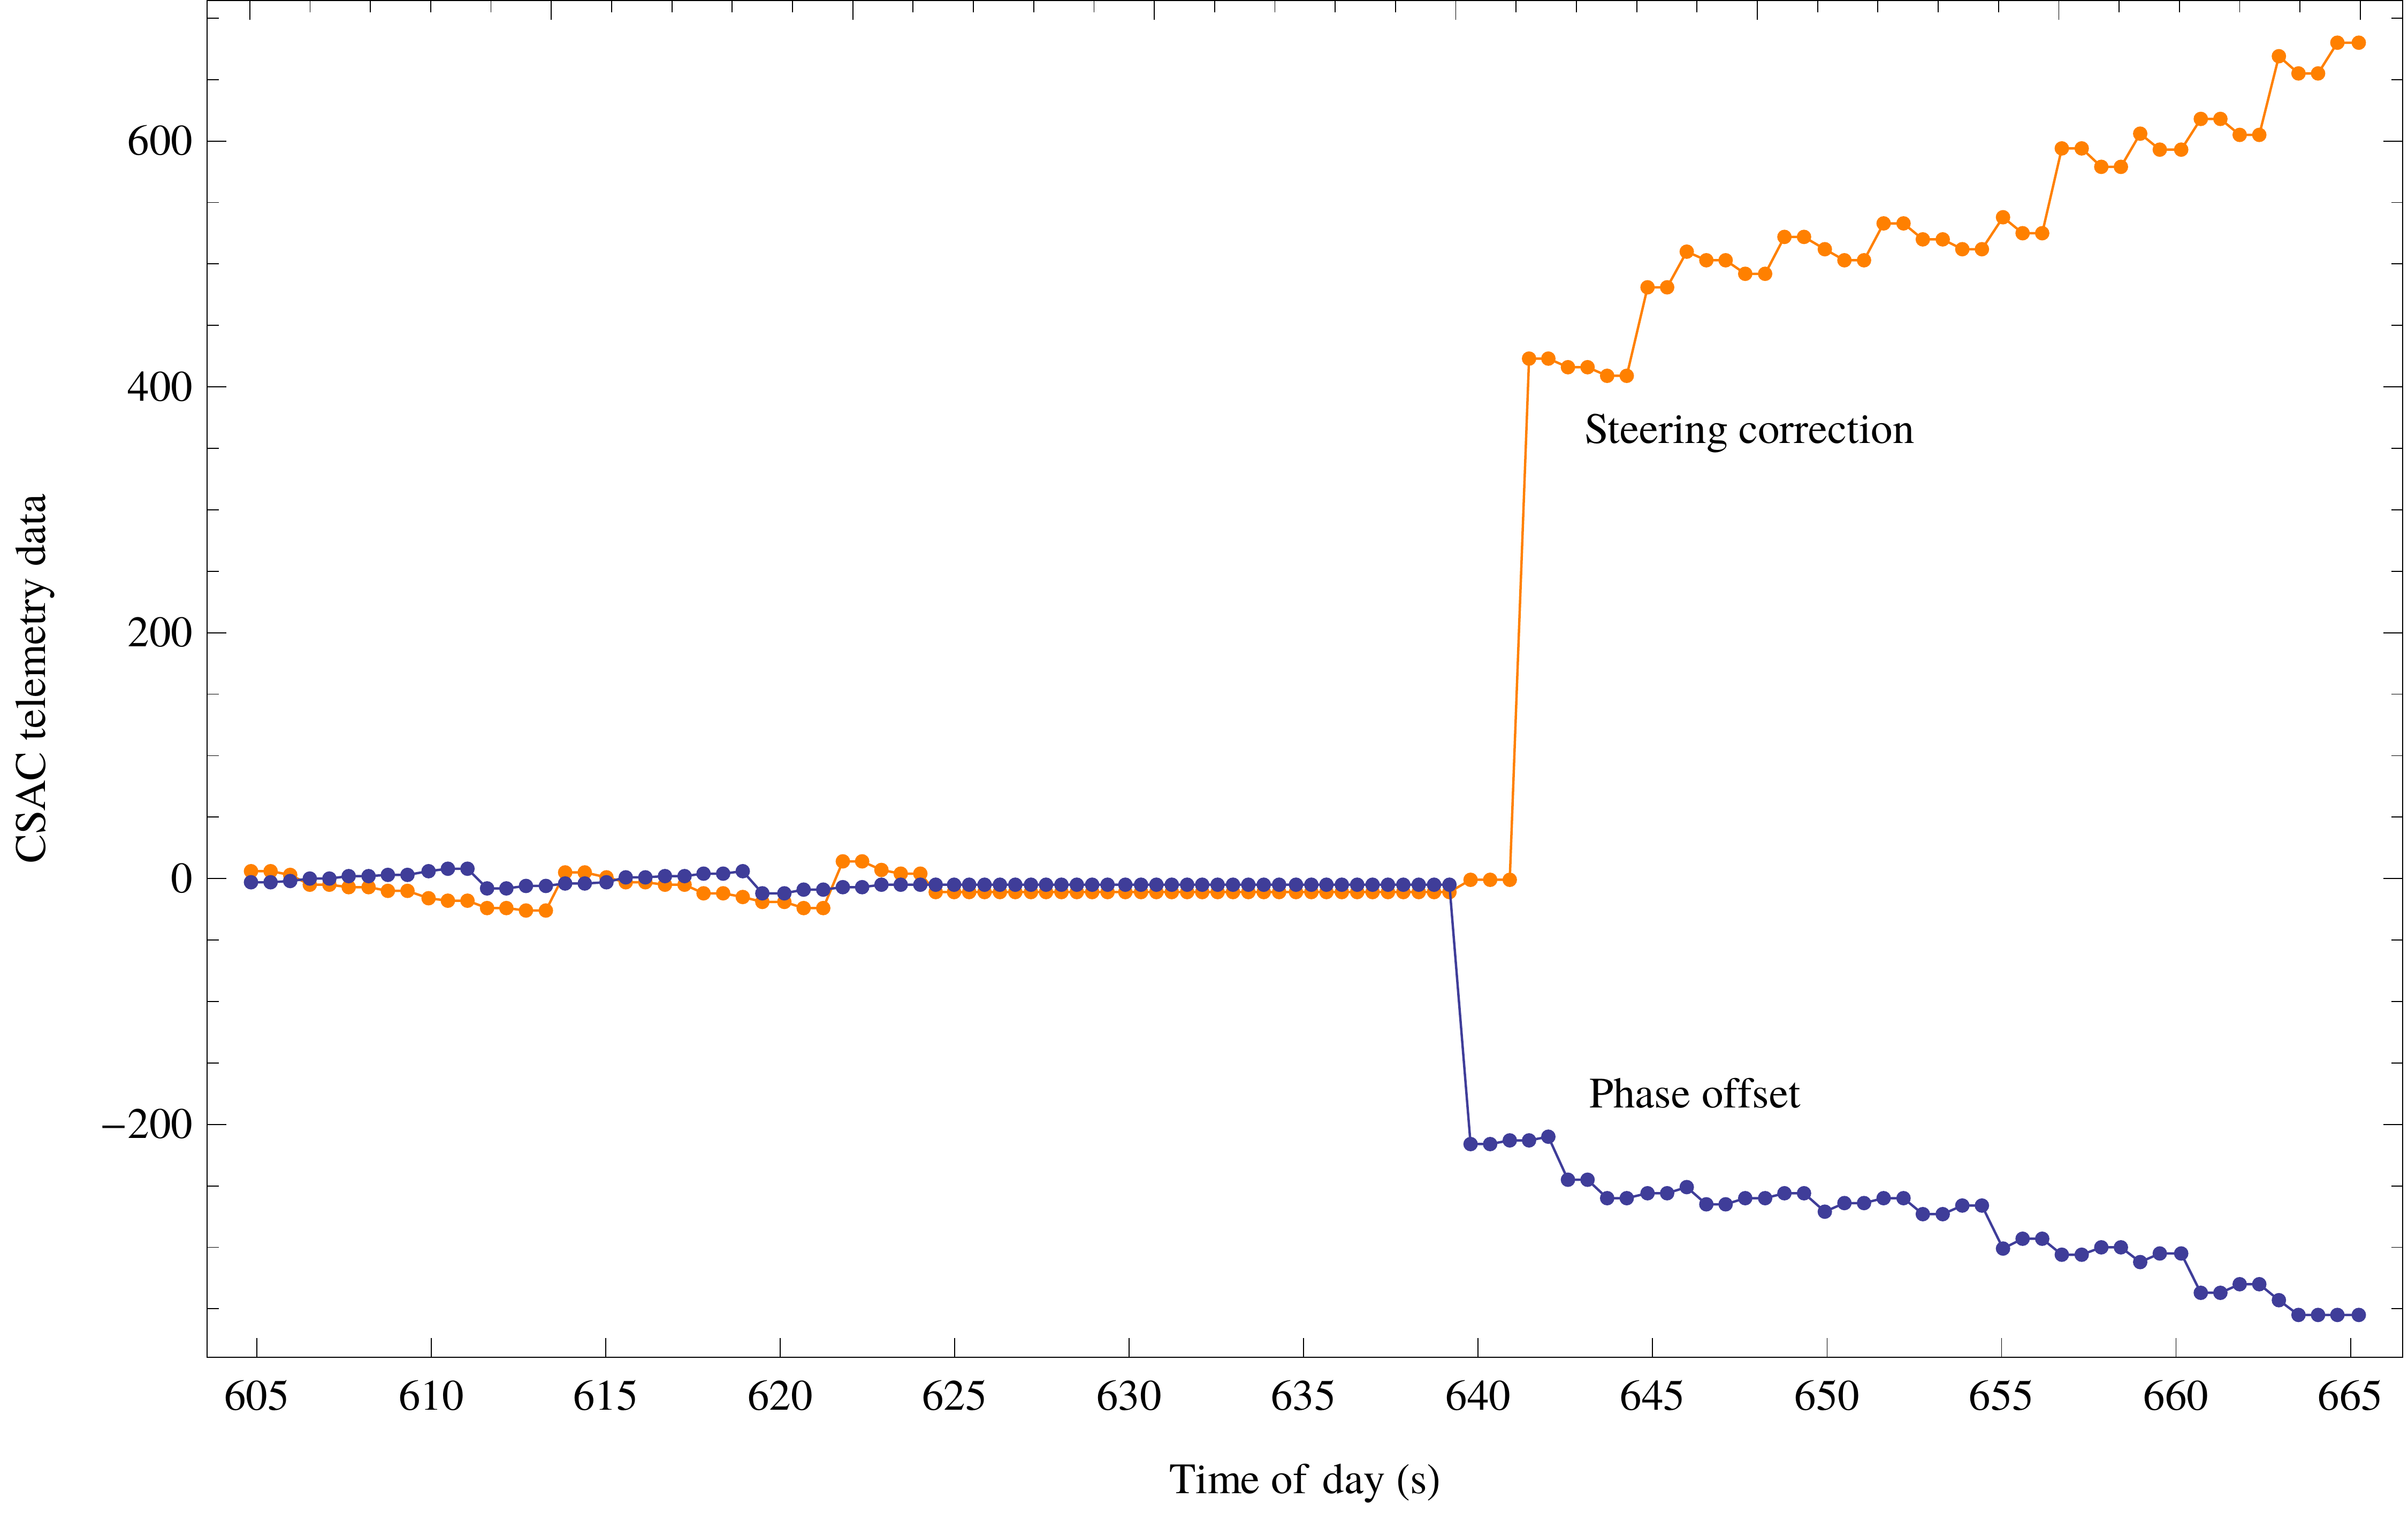
\includegraphics[scale=0.70]{thesis/graphics/disturbance57667-csac-telemetry-phase-steer-combined-zoom-in-2-1.png}
        \caption{Måleserie gjort under utilsiktet forstyrrelse}
      \end{figure}
\end{frame}

\section{Konklusjon}
\begin{frame}
  \frametitle{Konklusjon}
  \begin{itemize}
    \setlength\itemsep{2em}
    \item Effektiv deteksjon 
    \begin{itemize}
      \item Vanskelig å spoofe to mottakere
      \item God klokke -- litte spillerom for narring
    \end{itemize}
    \item Effektivitet til Sensor Server arkitekturen. 
    \begin{itemize}
      \item Lav responstid
      \item Høy stabilitet 
      \item Enkel å bygge ut med flere sensorer
    \end{itemize}
  \end{itemize}
\end{frame}

\section{Videre arbeid}
\begin{frame}
    \frametitle{Videre arbeid}
  \begin{itemize}
      \setlength\itemsep{2em}
  \item Kommunikasjon med atomklokke
    \begin{itemize}
      \item CSAC fastvare problem?
    \end{itemize}
  \item Integrasjon av filtre
  \end{itemize}
\end{frame}

\section{Bibliografi}
\begin{frame}[allowframebreaks]%in case more than 1 slide needed
  \frametitle{Bibliografi}
  \printbibliography[heading=bibintoc]
\end{frame}

\end{document}